% Options for packages loaded elsewhere
\PassOptionsToPackage{unicode}{hyperref}
\PassOptionsToPackage{hyphens}{url}
\PassOptionsToPackage{dvipsnames,svgnames*,x11names*}{xcolor}
%
\documentclass[
  12pt,
]{book}
\usepackage{lmodern}
\usepackage{setspace}
\usepackage{amssymb,amsmath}
\usepackage{ifxetex,ifluatex}
\ifnum 0\ifxetex 1\fi\ifluatex 1\fi=0 % if pdftex
  \usepackage[T1]{fontenc}
  \usepackage[utf8]{inputenc}
  \usepackage{textcomp} % provide euro and other symbols
\else % if luatex or xetex
  \usepackage{unicode-math}
  \defaultfontfeatures{Scale=MatchLowercase}
  \defaultfontfeatures[\rmfamily]{Ligatures=TeX,Scale=1}
\fi
% Use upquote if available, for straight quotes in verbatim environments
\IfFileExists{upquote.sty}{\usepackage{upquote}}{}
\IfFileExists{microtype.sty}{% use microtype if available
  \usepackage[]{microtype}
  \UseMicrotypeSet[protrusion]{basicmath} % disable protrusion for tt fonts
}{}
\makeatletter
\@ifundefined{KOMAClassName}{% if non-KOMA class
  \IfFileExists{parskip.sty}{%
    \usepackage{parskip}
  }{% else
    \setlength{\parindent}{0pt}
    \setlength{\parskip}{6pt plus 2pt minus 1pt}}
}{% if KOMA class
  \KOMAoptions{parskip=half}}
\makeatother
\usepackage{xcolor}
\IfFileExists{xurl.sty}{\usepackage{xurl}}{} % add URL line breaks if available
\IfFileExists{bookmark.sty}{\usepackage{bookmark}}{\usepackage{hyperref}}
\hypersetup{
  pdftitle={Cambios en la Cohesión Social en Chile},
  pdfauthor={Equipo CEPAL-ELSOC},
  colorlinks=true,
  linkcolor=blue,
  filecolor=Maroon,
  citecolor=Blue,
  urlcolor=Blue,
  pdfcreator={LaTeX via pandoc}}
\urlstyle{same} % disable monospaced font for URLs
\usepackage[left=4cm, right=3cm, top=2.5cm, bottom=2.5cm]{geometry}
\usepackage{longtable,booktabs}
% Correct order of tables after \paragraph or \subparagraph
\usepackage{etoolbox}
\makeatletter
\patchcmd\longtable{\par}{\if@noskipsec\mbox{}\fi\par}{}{}
\makeatother
% Allow footnotes in longtable head/foot
\IfFileExists{footnotehyper.sty}{\usepackage{footnotehyper}}{\usepackage{footnote}}
\makesavenoteenv{longtable}
\usepackage{graphicx,grffile}
\makeatletter
\def\maxwidth{\ifdim\Gin@nat@width>\linewidth\linewidth\else\Gin@nat@width\fi}
\def\maxheight{\ifdim\Gin@nat@height>\textheight\textheight\else\Gin@nat@height\fi}
\makeatother
% Scale images if necessary, so that they will not overflow the page
% margins by default, and it is still possible to overwrite the defaults
% using explicit options in \includegraphics[width, height, ...]{}
\setkeys{Gin}{width=\maxwidth,height=\maxheight,keepaspectratio}
% Set default figure placement to htbp
\makeatletter
\def\fps@figure{htbp}
\makeatother
\setlength{\emergencystretch}{3em} % prevent overfull lines
\providecommand{\tightlist}{%
  \setlength{\itemsep}{0pt}\setlength{\parskip}{0pt}}
\setcounter{secnumdepth}{5}
\usepackage[utf8]{inputenc}
\usepackage[spanish,es-tabla]{babel}
\usepackage[fixlanguage]{babelbib}
\usepackage{geometry}
\geometry{letterpaper,left=2cm,top=2cm, right=2cm}
\usepackage{times}           
\usepackage{caption}
\captionsetup[figure, table]{labelfont={bf},labelformat={default},labelsep=period}
\usepackage{graphicx}
\usepackage{float}
\usepackage{booktabs}
\usepackage{longtable}
\usepackage{array}
\usepackage{multirow}
\usepackage{wrapfig}
\usepackage{float}
\usepackage{colortbl}
\usepackage{xcolor}
\usepackage{pdflscape}
\usepackage{tabu}
\usepackage{threeparttable}
\usepackage{pdfpages} %para pdf portada

% fuente: https://stackoverflow.com/questions/45963505/coverpage-and-copyright-notice-before-title-in-r-bookdown
%\let\oldmaketitle\maketitle 
%\AtBeginDocument{\let\maketitle\relax}

% \renewcommand{\tablename}{Tabla}
% \ifxetex
%   \usepackage{polyglossia}
%   \setmainlanguage{spanish}
%   % Tabla en lugar de cuadro
%   \gappto\captionsspanish{\renewcommand{\tablename}{Tabla}
%           \renewcommand{\listtablename}{Índice de tablas}}
% \else
%   % \usepackage[spanish,es-tabla]{babel}
% \fi
\usepackage{booktabs}
\usepackage{longtable}
\usepackage{array}
\usepackage{multirow}
\usepackage{wrapfig}
\usepackage{float}
\usepackage{colortbl}
\usepackage{pdflscape}
\usepackage{tabu}
\usepackage{threeparttable}
\usepackage{threeparttablex}
\usepackage[normalem]{ulem}
\usepackage{makecell}
\usepackage{xcolor}

\title{Cambios en la Cohesión Social en Chile}
\author{Equipo CEPAL-ELSOC}
\date{2021-08-08}

\begin{document}
\maketitle

{
\hypersetup{linkcolor=}
\setcounter{tocdepth}{1}
\tableofcontents
}
\listoftables
\listoffigures
\setstretch{1.5}
\hypertarget{presentaciuxf3n}{%
\chapter*{Presentación}\label{presentaciuxf3n}}
\addcontentsline{toc}{chapter}{Presentación}

Este reporte de investigación consiste en un análisis de medición y cambios en la cohesión social en Chile en base a indicadores de la Encuesta Longitudinal Social de Chile - \href{https://coes.cl/encuesta-panel/}{ELSOC}, producida por \href{https://coes.cl/}{COES}

Autores:

\begin{itemize}
\tightlist
\item
  Juan Carlos Castillo
\item
  Emmanuelle Barozet
\item
  Vicente Espinoza
\end{itemize}

Ayudante de investigación: Kevin Carrasco.

\hypertarget{introducciuxf3n}{%
\chapter*{Introducción}\label{introducciuxf3n}}
\addcontentsline{toc}{chapter}{Introducción}

El Centro de Estudios de Conflicto y Cohesión Social (COES) realiza desde el año 2016 el primer ``Estudio Longitudinal Social de Chile'' (ELSOC). Este estudio consiste en encuestar a casi 3.000 chilenos, anualmente, a lo largo de una década. Por lo tanto, el diseño de ELSOC es cuantitativo de tipo panel, es decir, que se repite su aplicación año a año.

El principal objetivo de ELSOC es evaluar la manera como piensan, sienten y se comportan los chilenos en torno a un conjunto de temas referidos al conflicto y la cohesión social en Chile. Además, permite comparar la estabilidad o cambio en diversas dimensiones sociales atendiendo a factores que los moderan o explican a lo largo de los años.

Esta encuesta es aplicada por medio de un cuestionario estructurado que posee 7 módulos diferentes: Territorio, Redes y actitudes sociales, Ciudadanía y democracia, Desigualdad y legitimidad, Conflicto social, Salud y bienestar y Caracterización sociodemográfica. Posee un muestreo probabilístico, estratificado (por tamaño de ciudades), por conglomerados y multietápico (aleatorio en todas sus etapas): Se eligieron aleatoriamente 40 ciudades con más de 10.000 habitantes (92 comunas de 13 regiones), dentro de estas se escogieron aleatoriamente 1067 manzanas. Dentro de cada manzana se escogieron hogares aleatoriamente y dentro de cada hogar fueron elegidos aleatoriamente individuos con 18 años o más. Por lo tanto, su unidad básica de observación son personas individuales. Asimismo, la población objetivo son hombres y mujeres de 18 a 75 años. Esta encuesta alcanza un 77\% de representatividad de la población total del país y un 93\% de la población urbana, con un error muestral del 2\%. La muestra alcanzada en 2019 posee las respuestas de 3417 individuos, que incluye respuestas de participantes de la primera ola (2016) y de la muestra de refresco iniciada en 2018 (COES, \protect\hyperlink{ref-coes_Radiografia_2019}{2019}).

\hypertarget{mediciuxf3n-de-cohesiuxf3n-social-con-indicadores-elsoc}{%
\chapter{Medición de cohesión social con indicadores ELSOC}\label{mediciuxf3n-de-cohesiuxf3n-social-con-indicadores-elsoc}}

El objetivo de este primer capítulo es generar indicadores de cohesión social basados en el modelo conceptual de CEPAL, en particular para los denominados \emph{elementos constitutivos de la cohesión social} y que se presenta en la Figura \ref{fig:esquema-cepal}.

\begin{figure}[H]

{\centering 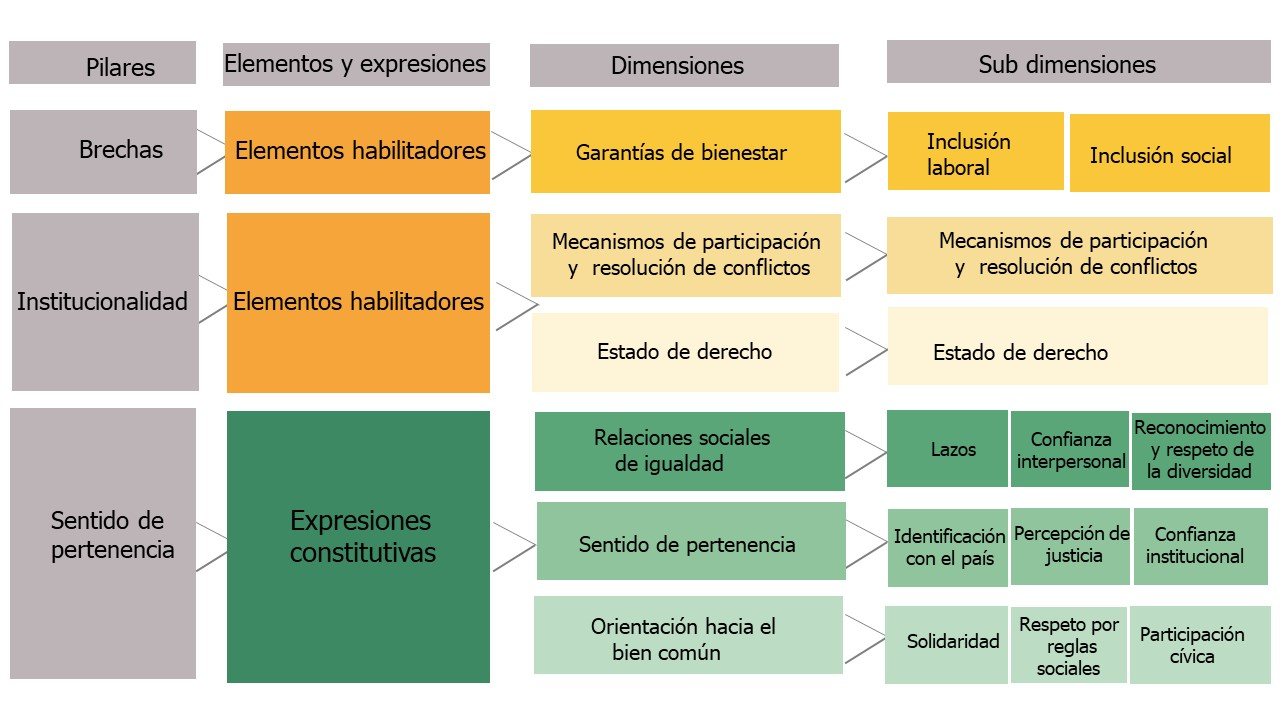
\includegraphics[width=1\linewidth,height=1\textheight]{images/dimensiones-cepal} 

}

\caption{Resumen dimensiones CEPAL.}\label{fig:esquema-cepal}
\end{figure}

En este capítulo se seleccionarán indicadores de la encuesta ELSOC (Estudio Longitudinal Social de Chile) que se asocien al contenido de cada una de las subdimensiones del concepto de cohesión social. Por ejemplo, si consideramos la dimensión ``Relaciones Sociales de Igualdad'', comenzaremos con la subdimensión ``lazos'' identificando indicadores de la encuesta que representen este concepto, y con la información disponible elaboraremos una propuesta para cubrir cada subdimensión.

Antes de comenzar con el trabajo de análisis de subdimensiones e indicadores, es pertinente mencionar una pequeña nota sobre medición. En este contexto medición hace referencia a otorgar propiedades numéricas a ciertos atributos individuales. Este proceso por definición no es exacto y conlleva error, ya que muchos de los conceptos que se trabajan en ciencias sociales no se pueden medir directamente y se consideran por lo tanto constructos latentes (como clase, estatus, pertenencia, confianza, entre muchos otros). Gran parte del trabajo de validez de las mediciones se trata justamente de poder cuantificar y minimizar este error. Para esto no solo basta con un análisis de \emph{validez aparente}, referido a que el contenido de la medición parezca relacionarse con el concepto que se desea medir, sino también con las propiedades métricas del indicador, como variabilidad y covariabilidad/correlación con otras medidas asociadas. Es por ello que en medición muchas veces se utilizan indicadores múltiples para un mismo concepto, de modo de poder identificarlo y estimarlo de una manera más robusta con técnicas específicas de análisis de constructos latentes.

{[}evaluar si es necesario dar más detalles de medición{]}

La breve mención a aspectos de medición del párrafo anterior nos permite aclarar el orden y el sentido del análisis que se presenta a continuación. En algunos casos encontraremos indicadores únicos para subdimensiones, donde no existe mayor alternativa que discutir su validez aparente y esperar un bajo nivel de error de medición. En otros casos existen baterías de indicadores múltiples, donde se propondrán índices que representen de mejor manera los elementos comunes (covarianza) y que subyacen a la batería, para lo que se utilizarán técnicas de análisis factorial.

Las decisiones respecto de los indicadores de cohesión social variarán según sea el número de variables presentes por subdimension:

\begin{itemize}
\item
  1 variable: se considerará simplemente el puntaje de la variable
\item
  2 variables: se analizará la correlación entre ambas y sobre esta base se podrá proponer un promedio simple
\item
  3 variables: se analizará la matriz de correlaciones y el alfa de Cronbach como medida de consistencia interna que permita trabajar con el promedio. Esta medida otorga un número que va entre 0 y 1, donde el nivele convencionales para considerar consistencia es 0.7 o mayor.
\item
  4 variables o más: se realizará un análisis factorial exploratorio para evaluar la dimensionalidad subyacente a los indicadores, y en base a este análisis se podrán proponer puntajes factoriales como índices.
\end{itemize}

A continuación se presenta el análisis ordenado por dimensiones:

\begin{itemize}
\tightlist
\item
  Relaciones sociales de igualdad
\item
  Sentido de pertenencia
\item
  Orientación hacia el bien común
\end{itemize}

Además de estas dimensiones del modelo de la CEPAL también se agrega una cuarta de cohesión social en el territorio, que se asocia a la confianza en vecinos, identificación barrial, sociabilidad barrial y satisfacción residencial.

\hypertarget{relaciones-sociales-de-igualdad}{%
\section{Relaciones sociales de igualdad}\label{relaciones-sociales-de-igualdad}}

De acuerdo a CEPAL, ``Esta parte de la definición de la cohesión social se acerca a aquellas que conciben la cohesión social como el compromiso y habilidad para trabajar juntos, incluso cuando los valores que poseen las personas sean distintos (Comisión Económica para África, 2016; Pornschlegel y Jürgensen, 2019; Dragolov y otros, 2013; De Beer, 2014; Woolcock, 2011; Banco Mundial, 2012, 2000; Stanley, 2003). Supone asimismo el principio de reconocimiento recíproco como precondición de la cohesión social (véase, por ejemplo, Jenson, 1998), así como la superación de todas las formas de discriminación.'' (CEPAL, \protect\hyperlink{ref-cepal_Cohesion_2021}{2021}, p. 45)

\textbf{Lazos}

Según CEPAL (\protect\hyperlink{ref-cepal_Cohesion_2021}{2021}), ``Los lazos sociales permiten generar espacios de cooperación que faciliten el desarrollo de relaciones sociales de igualdad, y establece patrones de reciprocidad interpersonal (PNUD, 2013)'' (p.~74)

El indicador propuesto en el informe de CEPAL es ``importancia de amigos en la vida'', que es un indicador de percepción de la Encuesta Mundial de Valores, a partir del cual se busca cuantificar la intensidad del tejido social en los países de la región. En el caso de ELSOC el indicador más cercano corresponde a ``Cantidad de amigos cercanos'', y que está presente solo en las olas 2 y 4. Un análisis descriptivo de este indicador, que sería el único representante de esta subdimensión, se presenta en la Figura \ref{fig:lazos}.

\begin{figure}[H]

{\centering 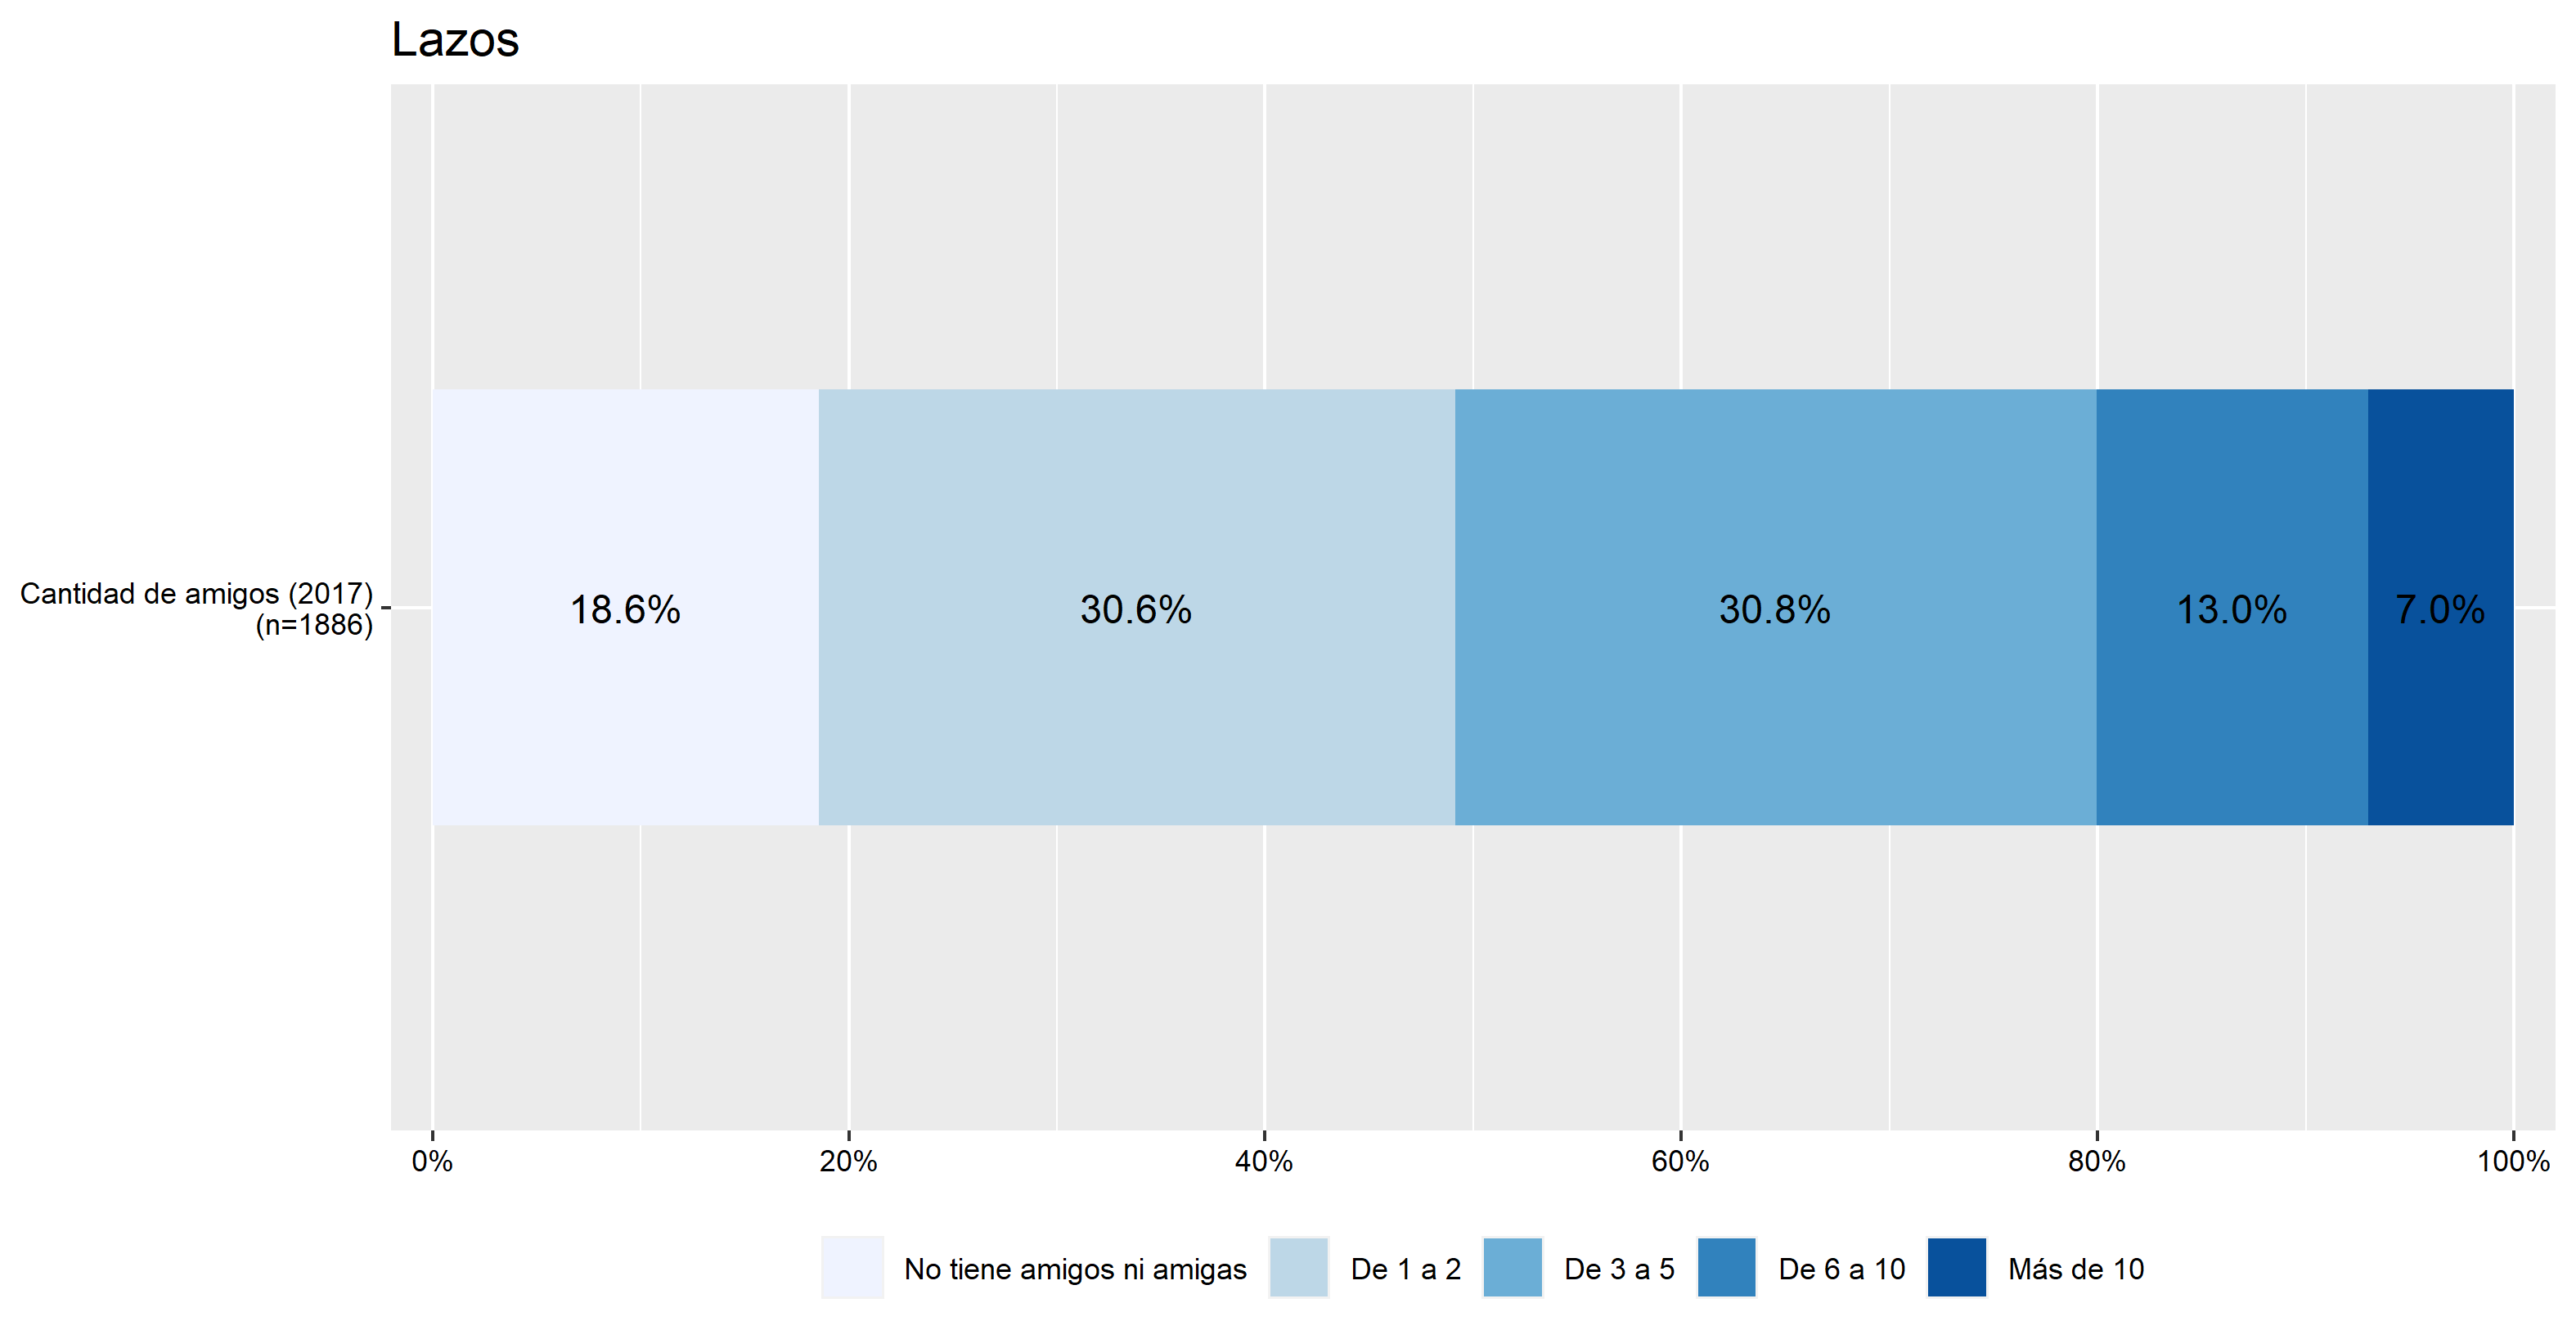
\includegraphics[width=1\linewidth,height=1\textheight]{output/graphs/lazos} 

}

\caption{Cantidad de amigos cercanos.}\label{fig:lazos}
\end{figure}

\textbf{Confianza interpersonal}

La confianza interpersonal es un atributo de las relaciones sociales que permite la interacción intergrupal y facilita la acción colectiva a favor de los objetivos compartidos. Por lo tanto, ``la confianza se considera un habilitador de la cooperación y participación (capital social)'' (CEPAL, \protect\hyperlink{ref-cepal_Cohesion_2021}{2021}, p. 74).

En el informe de CEPAL se utilizan los indicadores ``Confianza en la gente de su comunidad'', que busca cuantificar que tan confiable consideran a los habitantes de su comunidad y ``Confianza en la gente que se conoce por primera vez'', en el cual se cuantifica si se puede confiar en la mayoría de las personas o uno debe ser lo suficientemente cuidadoso con los demás. Al trabajar con ELSOC los indicadores que van en esta línea son ``Se puede confiar en la mayoría de las personas'', ``La mayoría de las personas tratan de ayudar a las demás'' y ``la mayoría de la gente trata de ser justa'', presentes en las cuatro olas. Un análisis descriptivo de estos indicadores se presentan en la Figura \ref{fig:confianza-interpersonal} y un análisis bivariado en la Figura \ref{fig:confianza-interpersonal-cor}.

\begin{figure}[H]

{\centering 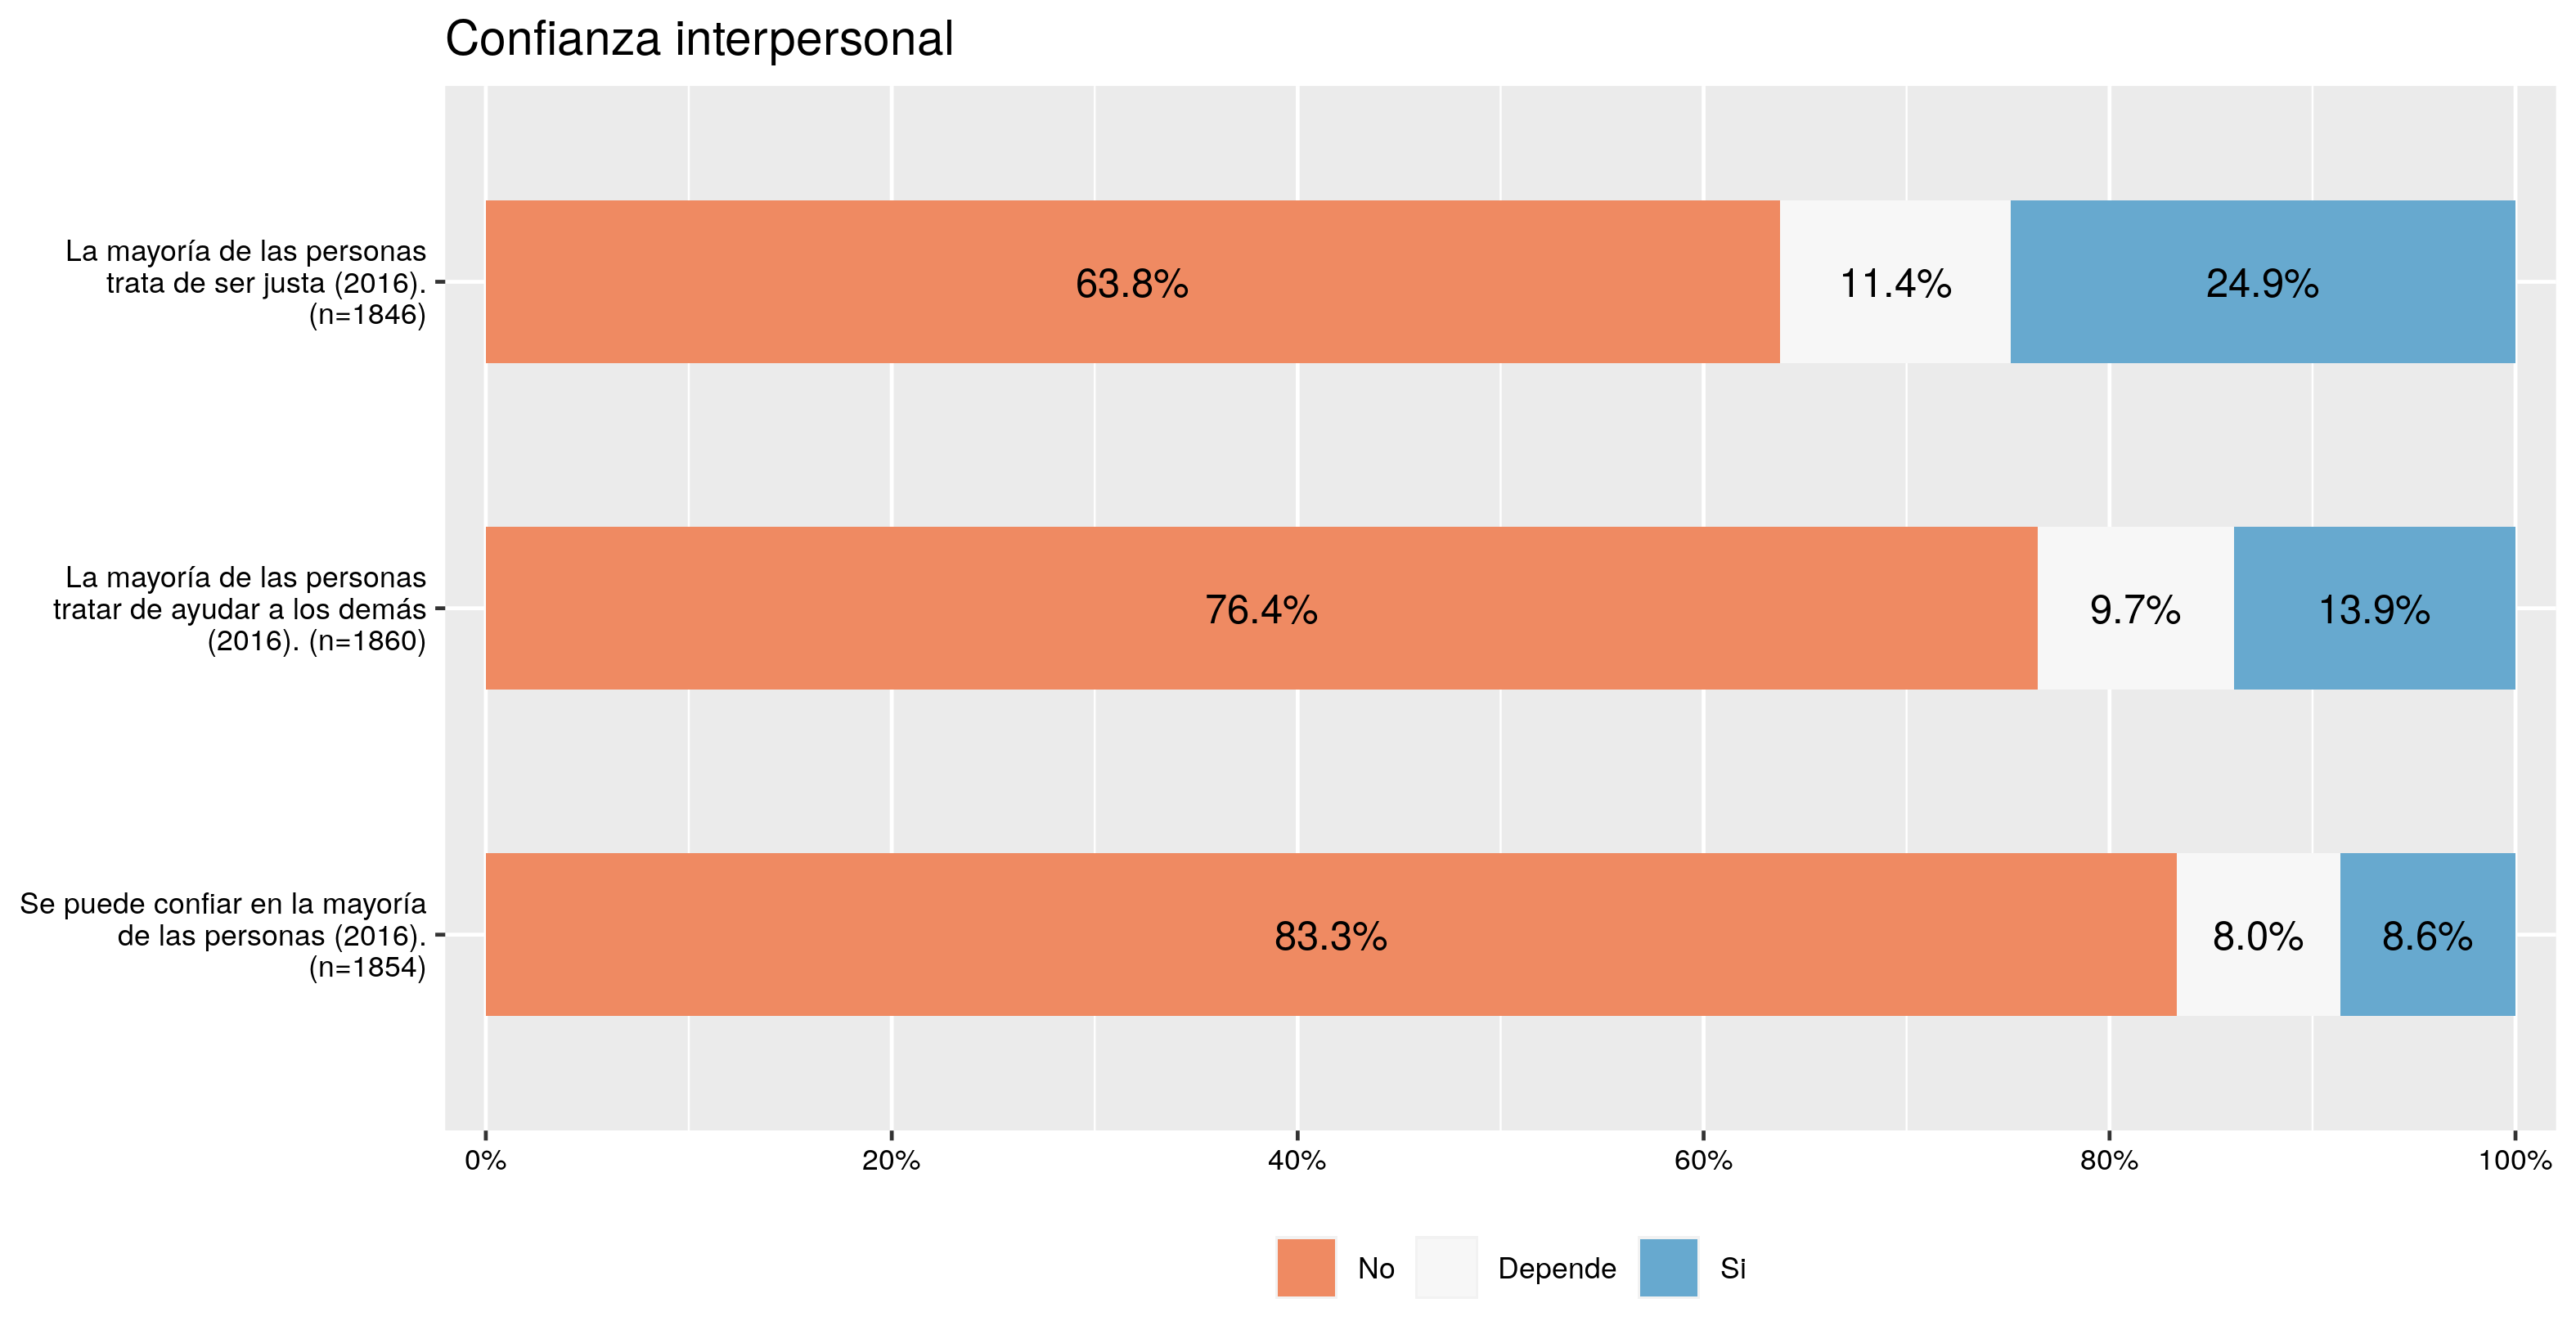
\includegraphics[width=1\linewidth,height=1\textheight]{output/graphs/confianza-interpersonal} 

}

\caption{Confianza interpersonal.}\label{fig:confianza-interpersonal}
\end{figure}

En la matriz de correlaciones de la Figura \ref{fig:confianza-interpersonal-cor} vemos que las correlaciones entre los indicadores van en el rango bajo a moderado, donde los indicadores más correlacionados son A y B. Al calcular la consistencia interna de estos indicadores mediante alpha de Cronbach el resultado arroja 0.45, bastante por debajo del límite recomendable de 0.7. Por lo tanto, el índice sugerido para esta subdimensión considera un promedio solo de aquellos items que presentan una correlación mayor: ``Se puede confiar en la mayoría de las personas'' y ``la mayoría de las personas trata de ayudar a los demás''.

\begin{figure}[H]

{\centering 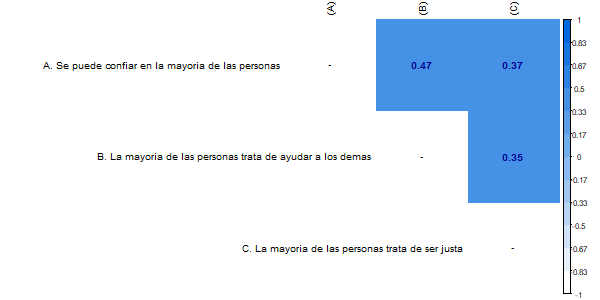
\includegraphics[width=1\linewidth,height=1\textheight]{output/graphs/confianza-interpersonal_cor} 

}

\caption{Asociación indicadores Confianza interpersonal.}\label{fig:confianza-interpersonal-cor}
\end{figure}

\textbf{Reconocimiento y respeto de la diversidad}

Las relaciones sociales de igualdad suponen el reconocimiento de la dignidad del ``otro'' y el reconocimiento de ser parte de una comunidad de iguales en materia de derechos ciudadanos, siendo un elemento que surge de la interacción en redes y asociaciones con individuos de distintas características (CEPAL, \protect\hyperlink{ref-cepal_Cohesion_2021}{2021}).

En el informe de CEPAL se utilizan dos indicadores en esta subdimensión: ``aprueba el derecho a contraer matrimonio de parejas del mismo sexo'', que se incluye con el objetivo de cuantificar la tolerancia hacia los individuos y comunidades con distinta orientación sexual y ``Los hombres no tienen prioridad sobre la mujer, a la hora acceder a un trabajo'', que se incluye con el objetivo de cuantificar la cultura de igualdad de género en la sociedad. Además, se deja como pendiente la construcción de un indicador sobre tolerancia a personas de distinta raza y etnia, así como de percepción de discriminación. En el caso de ELSOC encontramos indicadores distintos pero relacionados con actitudes hacia la diversidad: a) Chile pierde su identidad con la llegada de inmigrantes; b) con la llegada de inmigrantes aumenta el desempleo; c) grado de acuerdo con adopción homoparental; d) grado de confianza con personas homosexuales; e) grado de confianza con personas mapuche; y f) grado de confianza con personas inmigrantes. Los dos primeros indicadores están presentes en las cuatro olas, adopción homoparental en olas 3 y 4 y el resto de indicadores en las olas 2 y 4. Un análisis descriptivo de estos indicadores se presentan en la Figura \ref{fig:prejuicios} y en la Figura \ref{fig:diversidad} y un análisis bivariado en la Figura \ref{fig:diversidad-cor}.

\begin{figure}[H]

{\centering 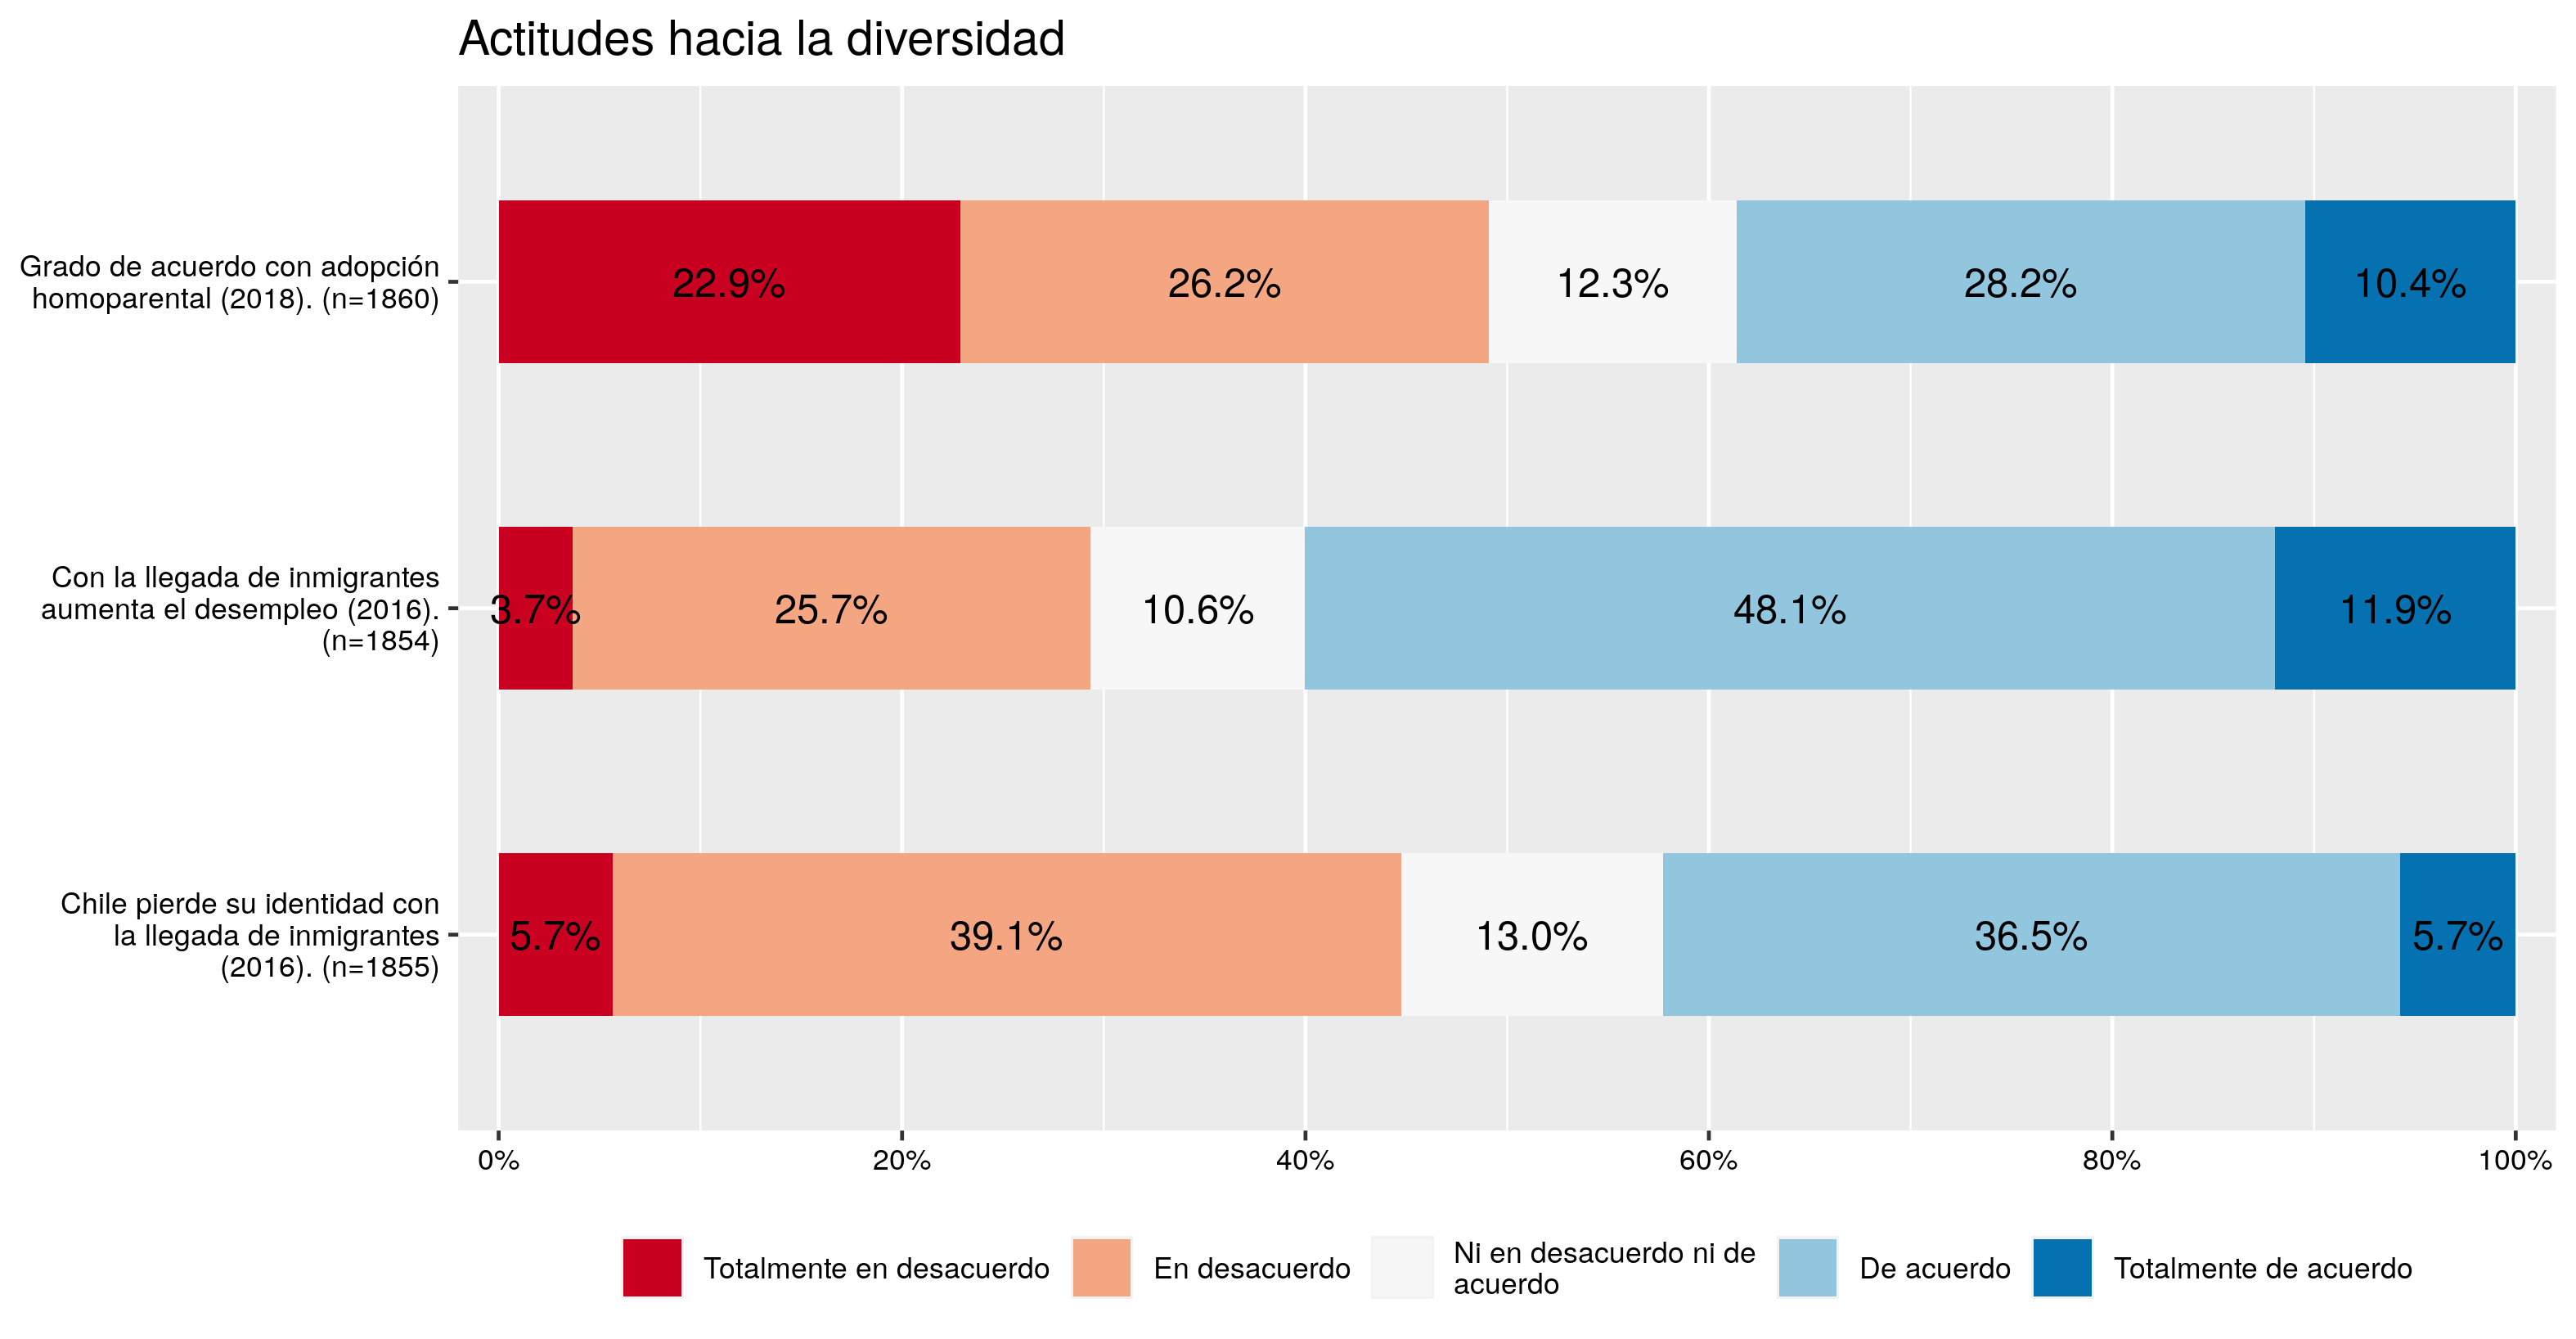
\includegraphics[width=1\linewidth,height=1\textheight]{output/graphs/prejuicios} 

}

\caption{Prejuicios hacia inmigrantes y adopción homoparental.}\label{fig:prejuicios}
\end{figure}

\begin{figure}[H]

{\centering 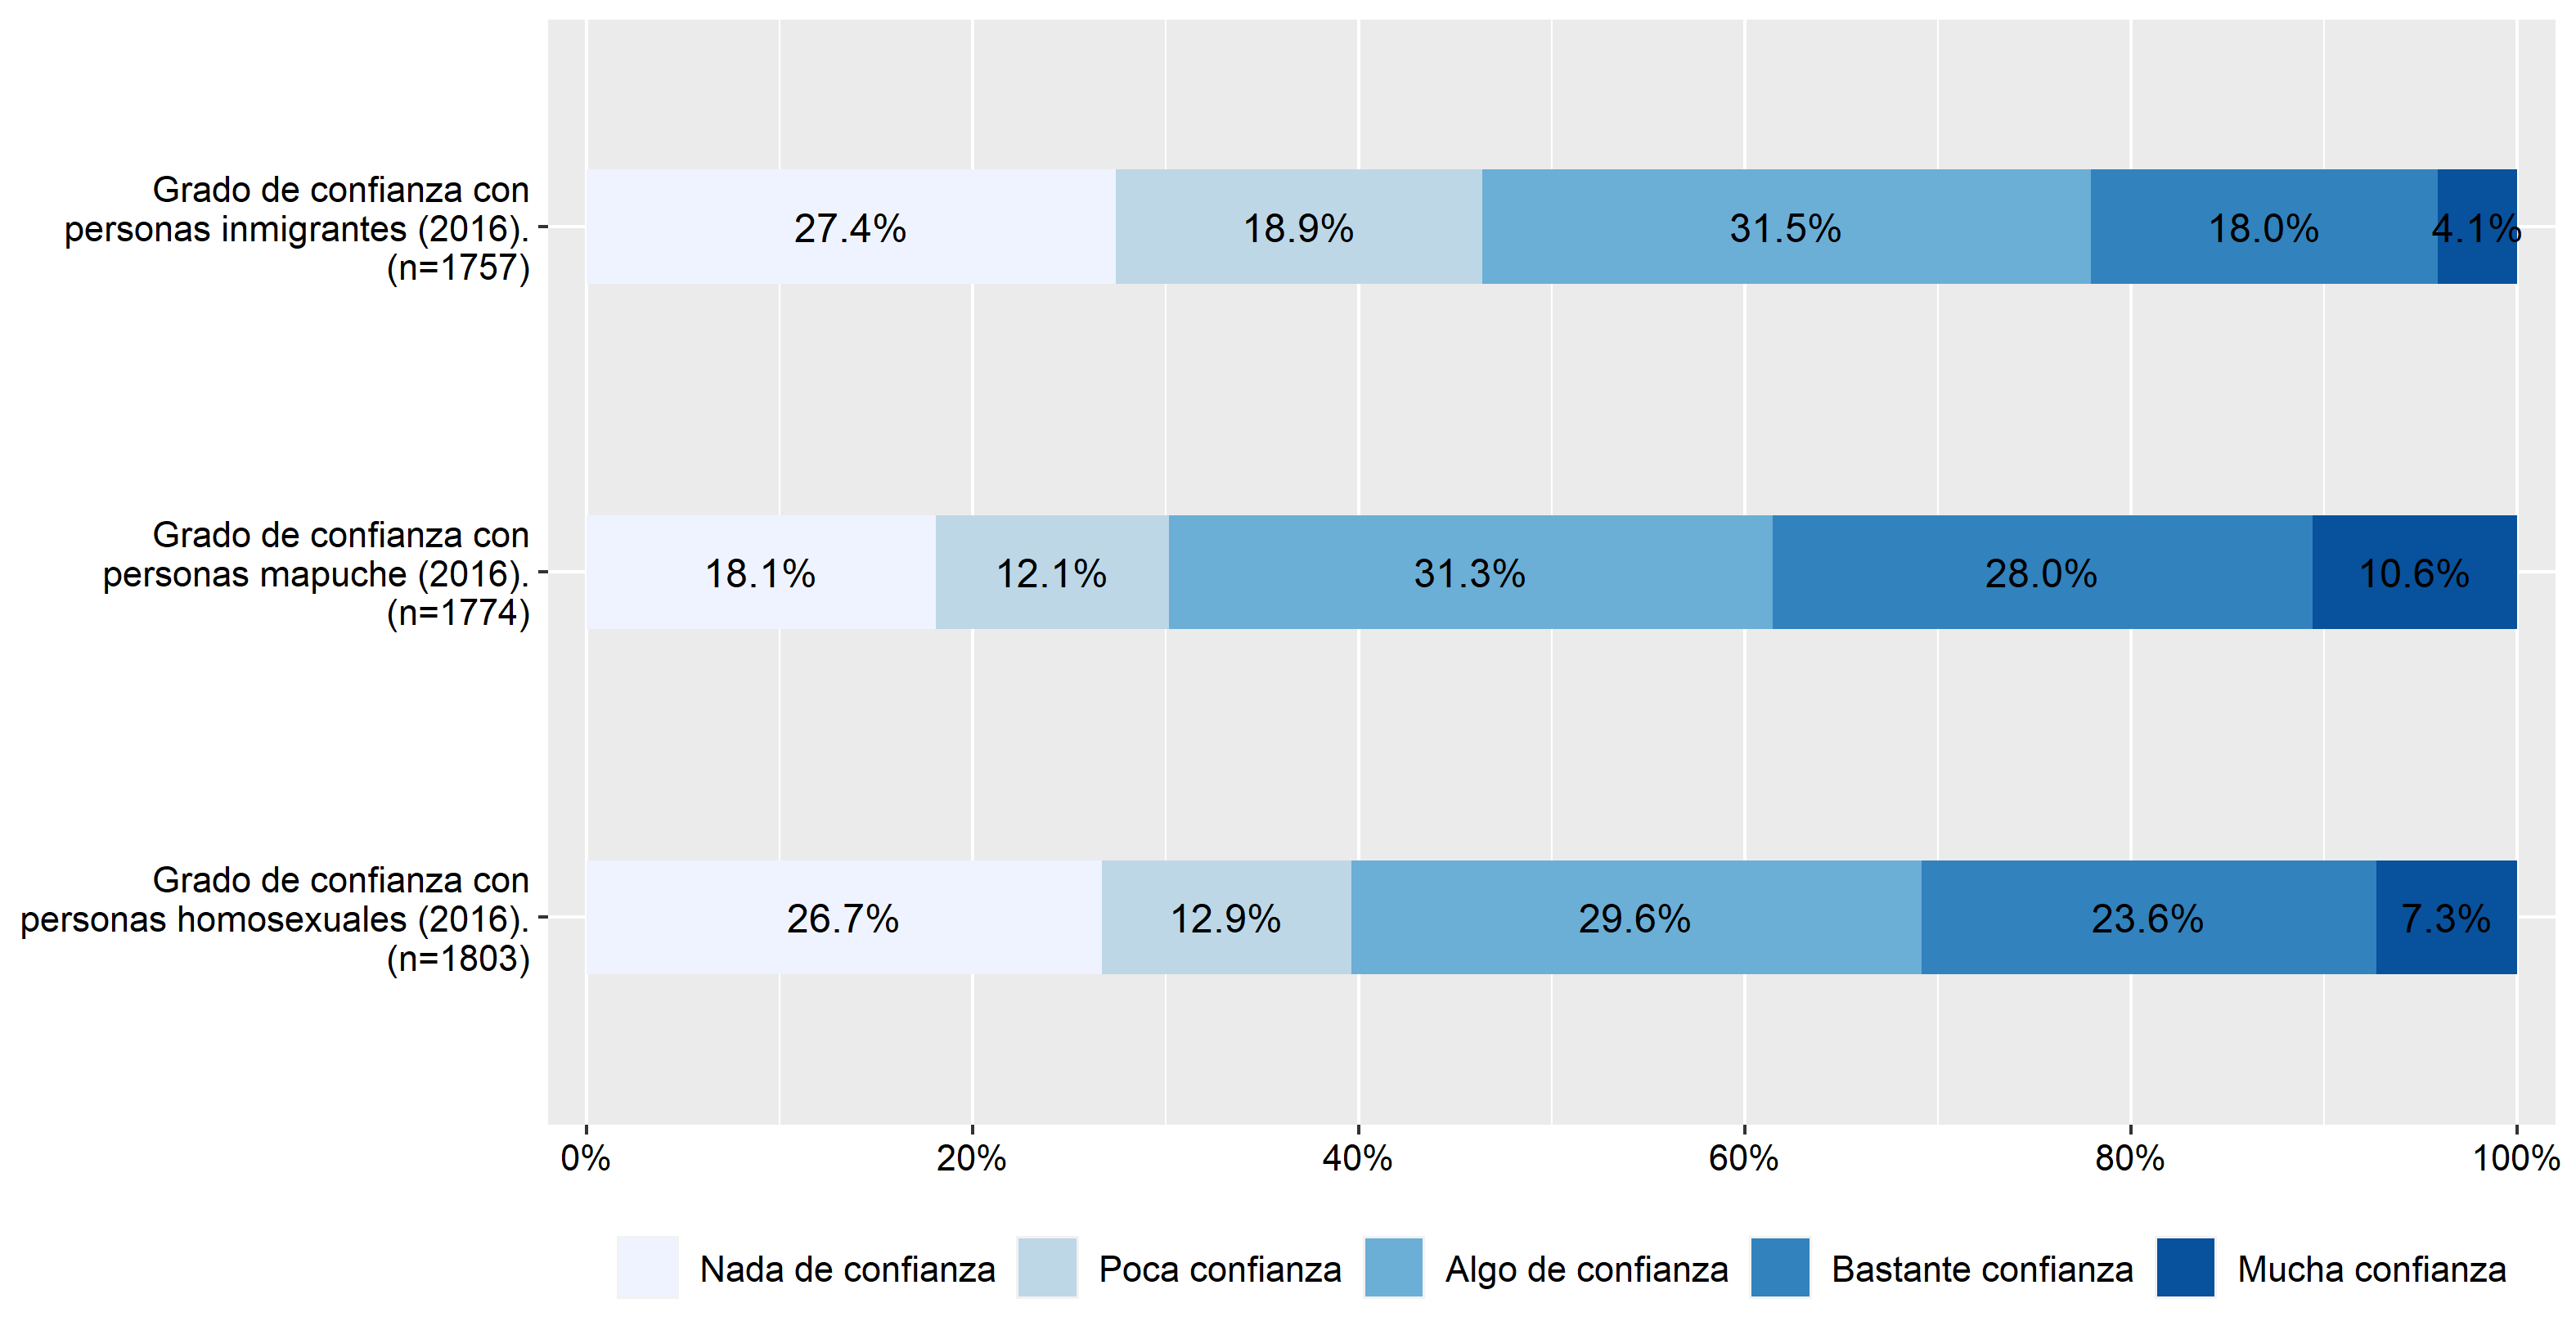
\includegraphics[width=1\linewidth,height=1\textheight]{output/graphs/diversidad} 

}

\caption{Grado de confianza grupos sociales.}\label{fig:diversidad}
\end{figure}

\begin{figure}[H]

{\centering 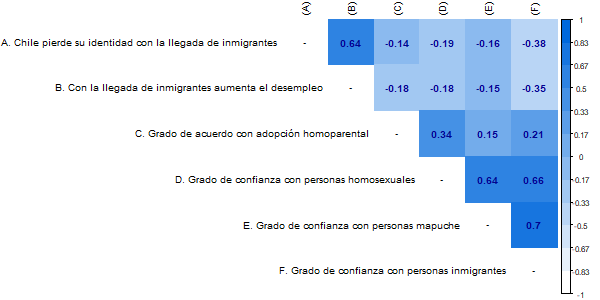
\includegraphics[width=1\linewidth,height=1\textheight]{output/graphs/diversidad_cor} 

}

\caption{Asociación indicadores Reconocimiento y respeto de la diversidad.}\label{fig:diversidad-cor}
\end{figure}

Para poder avanzar hacia la construcción de un índice basado en esta serie de indicadores utilizaremos análisis factorial exploratorio, que nos entrega información de las dimensiones comunes que subyacen a un conjunto de indicadores. La Tabla \ref{tab:div-fa} nos muestra el resultado de la extracción de tres factores:

\begin{longtable}[]{@{}l@{}}
\caption{\label{tab:div-fa}Dimensiones de reconocimiento y respeto de la diversidad.}\tabularnewline
\toprule
\endhead

\includegraphics[width=5.20833in,height=\textheight]{output/tables/div_fa.png}\tabularnewline
\bottomrule
\end{longtable}

En la Tabla \ref{tab:div-fa} observamos en la primera columna un factor que se relaciona con las preguntas sobre el grado de confianza de la Figura \ref{fig:diversidad}, luego un segundo factor asociado a las preguntas de inmigrantes, y finalmente un tercer factor asociado a la pregunta de adopción homoparental. Atendiendo ahora a la varianza asociada a estos factores (SS loadings), el primer factor representa casi un 30\% de la varianza, el segundo alrededor de 20\% y el tercero muy por debajo con 0.08. Por lo tanto podemos decir que hay mayor consistencia en los dos primeros factores, y entre ellos dos el asociado a diversidad es el más claro. Basándose en este análisis es posible proponer dos índices asociados a esta subdimensión y que serán calculados mediante puntajes factoriales: uno sobre diversidad y el otro sobre migrantes.

\hypertarget{sentido-de-pertenencia}{%
\section{Sentido de pertenencia}\label{sentido-de-pertenencia}}

Una segunda dimensión de la definición propuesta corresponde al sentido de pertenencia, que ``alude a la vinculación e identificación de las personas respecto a la sociedad y a las instituciones y grupos que los integran. Incluye los niveles micro, meso y macro.'' (CEPAL, \protect\hyperlink{ref-cepal_Cohesion_2021}{2021}, p. 45). Esta definición permite relevar la importancia de ``las dinámicas de reconocimiento y participación social para conducir procesos dinámicos de inclusión que contribuyan a la cohesión social y al logro del bienestar (véase, por ejemplo, Jenson, 1998; Kymlicka, 1998).'' (CEPAL, \protect\hyperlink{ref-cepal_Cohesion_2021}{2021}, p. 45).

\textbf{Identificación con el país}

Por medio de esta subdimensión, se busca cuantificar la identificación de los individuos ``con los valores y acciones que representan sus instituciones, y la concordancia con los propios'' (CEPAL, \protect\hyperlink{ref-cepal_Cohesion_2021}{2021}, p. 66).

En el informe CEPAL se incluyen los indicadores ``Orgullo por el sistema político'', que busca medir la adhesión de los encuestados con la labor que realizan sus instituciones en la representación de sus valores y objetivos y ``Orgullo por su nacionalidad'', que busca cuantificar la identificación de los encuestados con los valores y normas que rigen las instituciones del país. Al trabajar con ELSOC se utilizarán los indicadores ``Orgullo de ser chileno'' e ``Identificación con Chile'' que están presentes en las cuatro olas. Un análisis descriptivo de estos indicadores se presentan en la Figura \ref{fig:identificacion}. La correlación entre estos indicadores es positiva y alta (r=0.76).

\begin{figure}[H]

{\centering 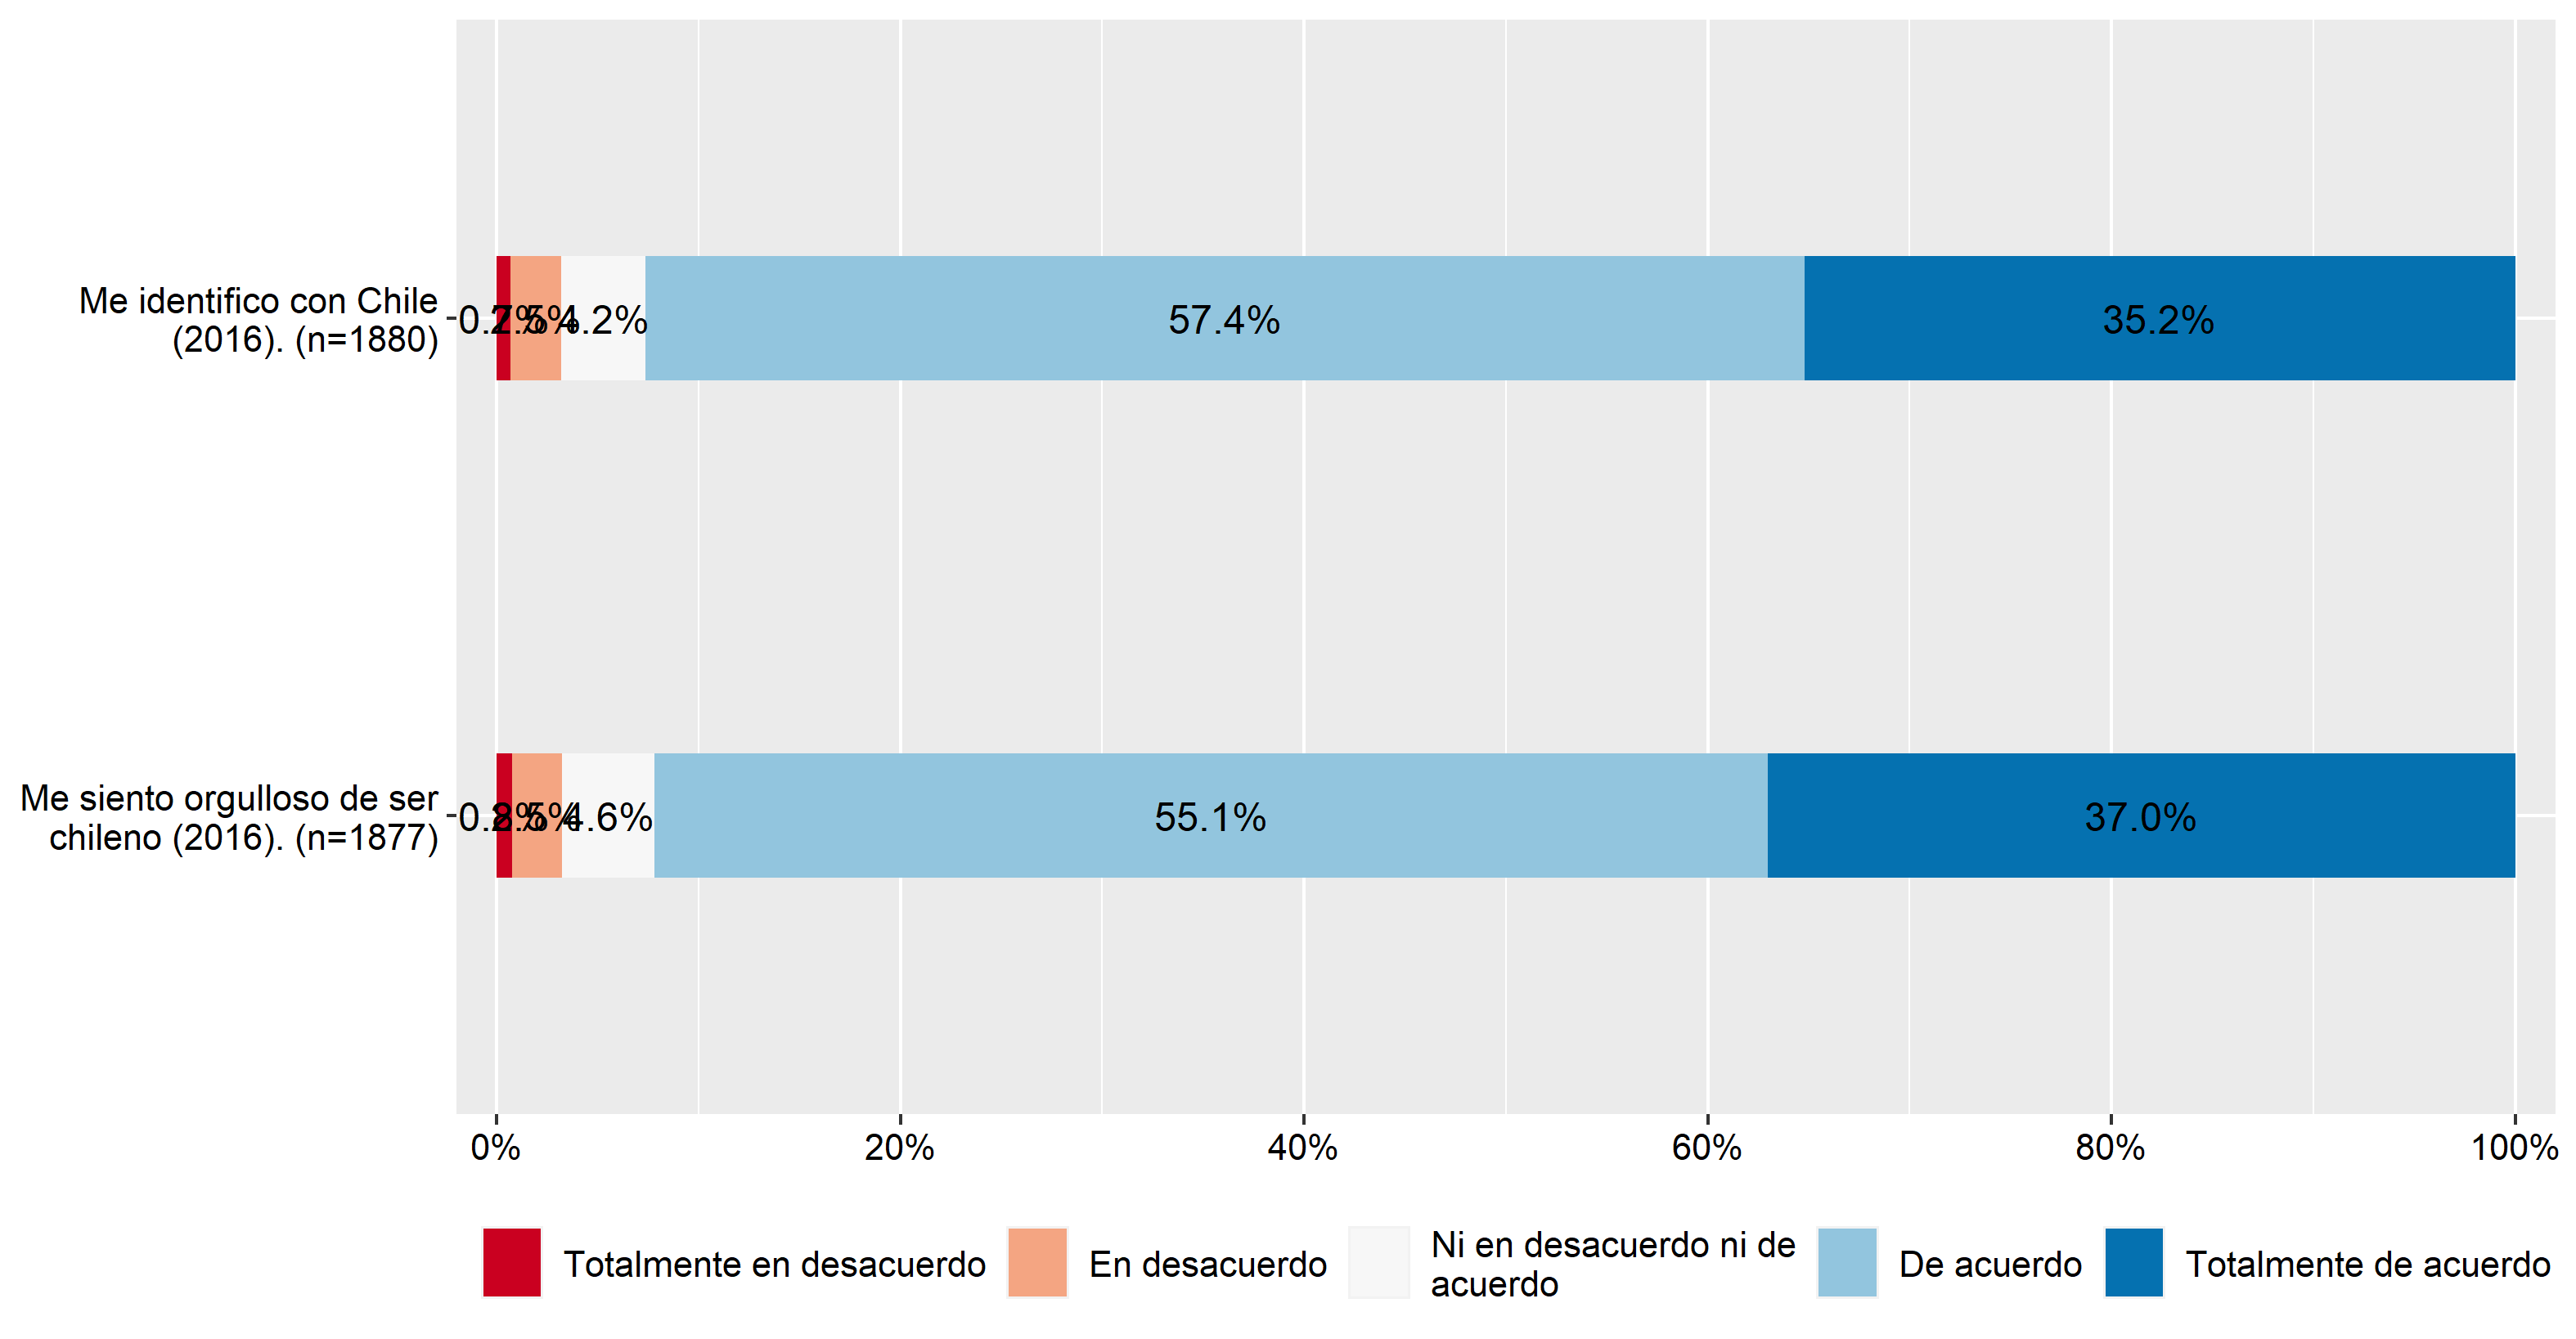
\includegraphics[width=1\linewidth,height=1\textheight]{output/graphs/identificacion} 

}

\caption{Identificación y orgullo con Chile.}\label{fig:identificacion}
\end{figure}

\textbf{Percepción de justicia}

La subdimensión de percepción de justicia refiere al examen que realizan los miembros de la sociedad respecto a la capacidad de las instituciones de entregar bienestar y/o distribuir el poder económico y político (CEPAL, \protect\hyperlink{ref-cepal_Cohesion_2021}{2021}).

En el informe de CEPAL se utilizan los indicadores ``Se deben equiparar los sueldos, no mantener desigualdad para incentivar el esfuerzo personal'', que cuantifica percepciones respecto a aversiones hacia la desigualdad; ``El trabajo a largo plazo da beneficios, no las conexiones o suerte'', que busca captar percepciones sobre la estructura de oportunidades en el país y las expectativas de movilidad social; y ``El Estado debe implementar políticas para reducir la desigualdad de ingreso'', que aborda las percepciones respecto a la desigualdad de ingresos en el país. Al trabajar con ELSOC se utilizan los indicadores ``En Chile las personas son recompensadas por su esfuerzo'' y ``En Chile las personas son recompensadas por su inteligencia'', presentes en todas las olas. Un análisis descriptivo de estos indicadores se presentan en la Figura \ref{fig:justicia}. La correlación entre estos indicadores es positiva y alta (r=0.7).

\begin{figure}[H]

{\centering 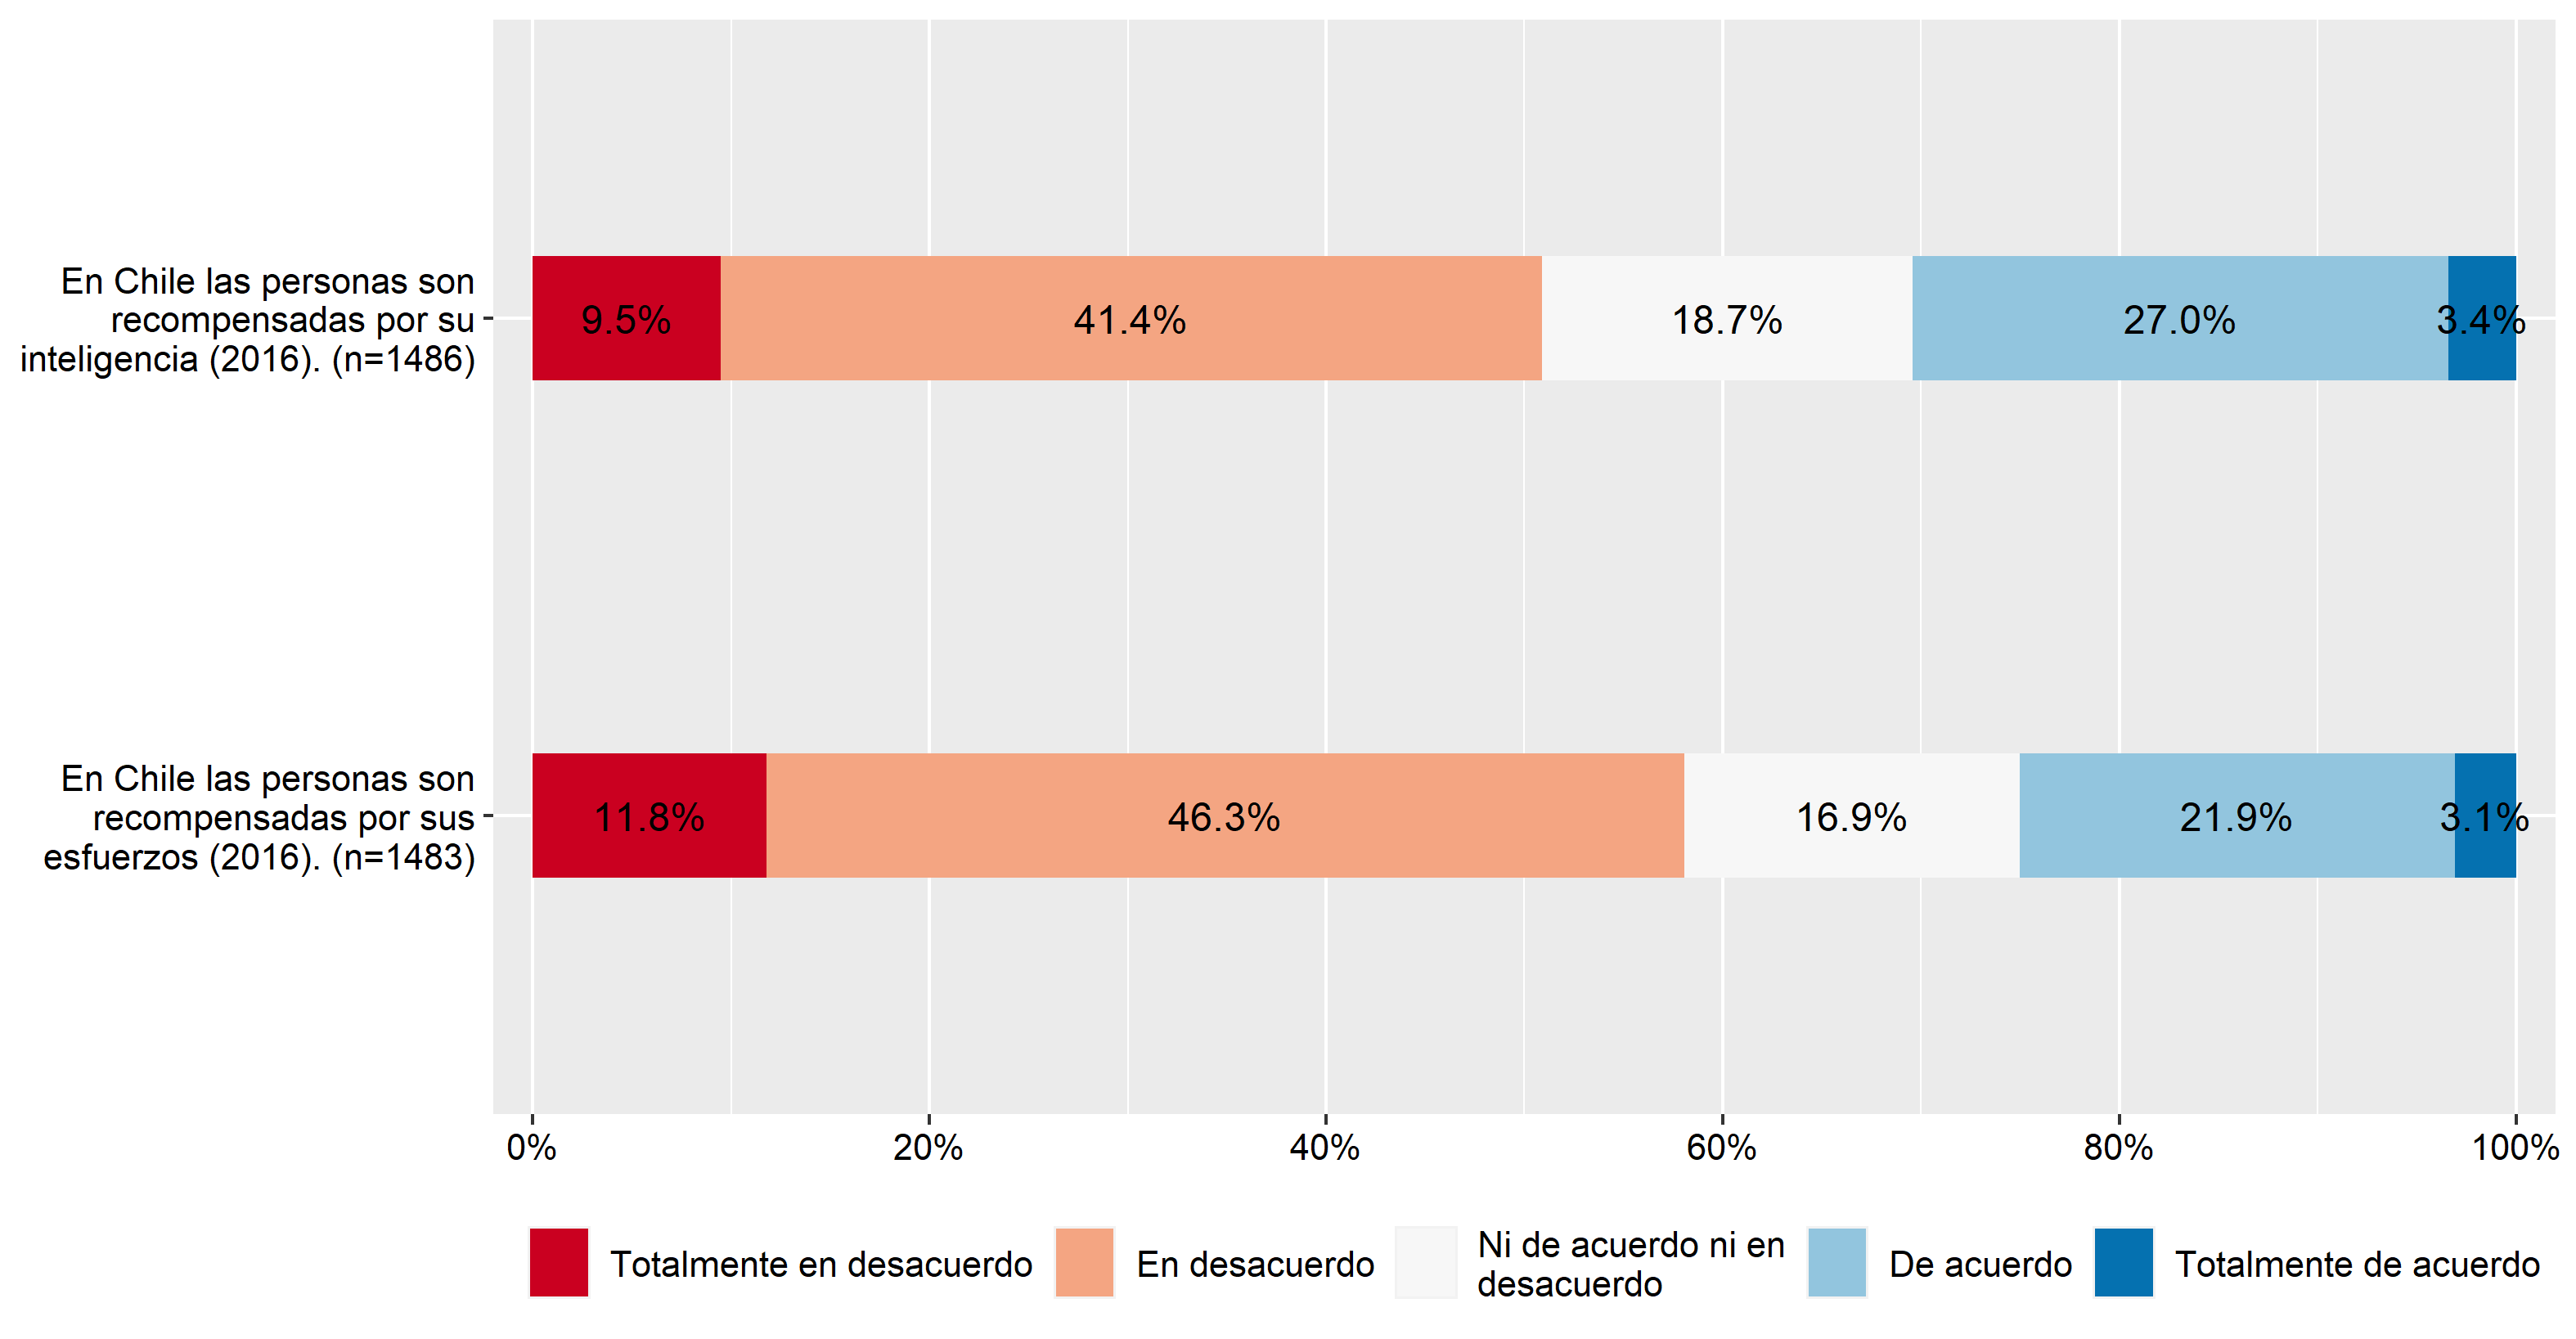
\includegraphics[width=1\linewidth,height=1\textheight]{output/graphs/justicia} 

}

\caption{Descriptivos Percepción de recompensa por esfuerzo e inteligencia.}\label{fig:justicia}
\end{figure}

\textbf{Confianza institucional}

La subdimensión de confianza institucional ``mide la valoración implícita de las acciones llevadas a cabo por las instituciones para representar los valores de la sociedad y/o de orientar la acción hacia el bien colectivo (Warren, 2010)'' (CEPAL, \protect\hyperlink{ref-cepal_Cohesion_2021}{2021}, p. 66).

En informe CEPAL utilizan grado de confianza en (a) las cortes, (b) el Congreso Nacional, (c) la Policía Nacional, (d) los partidos políticos, (e) el ejecutivo y (f) las elecciones. Al trabajar con ELSOC se utilizan los siguientes ocho indicadores que están presentes en las cuatro olas: grado de confianza en (a) el gobierno, (b) los partidos políticos; (c) carabineros; (d) los sindicatos; (e) el poder judicial; (f) las empresas privadas; (g) el congreso nacional; y (h) el presidente/a de la república. Un análisis descriptivo de estos indicadores se presentan en la Figura \ref{fig:confianza-institucional} y un análisis bivariado en la Figura \ref{fig:confianza-institucional-cor}.

\begin{figure}[H]

{\centering 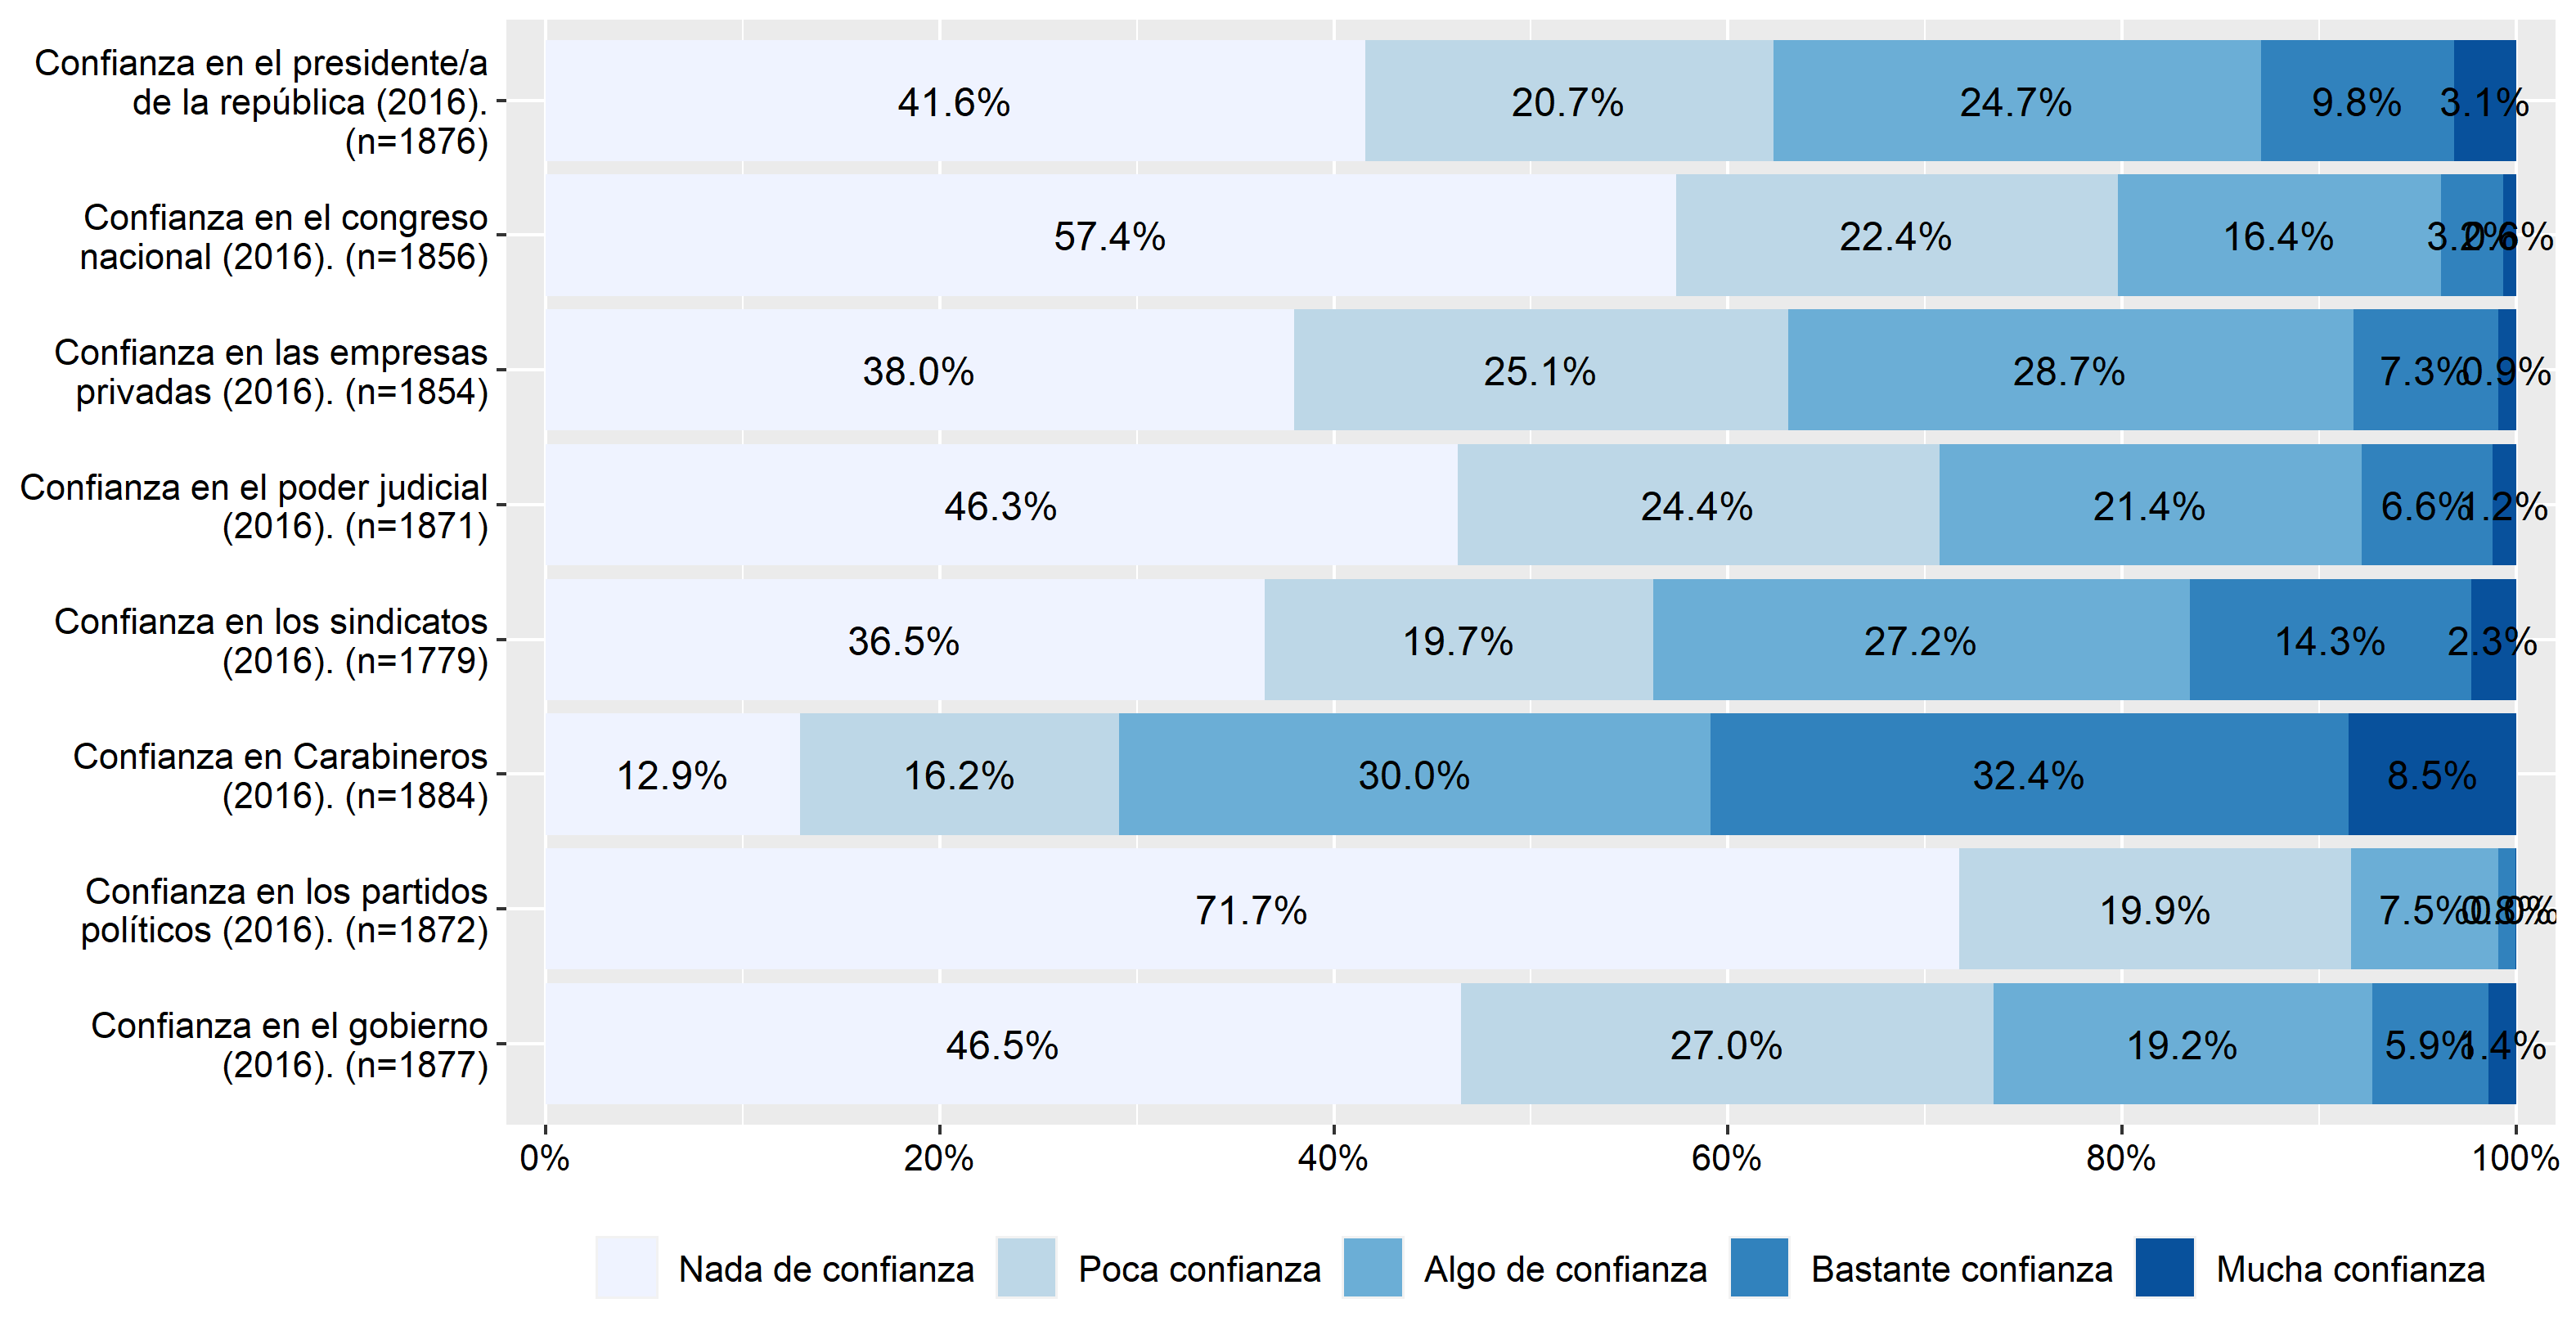
\includegraphics[width=1\linewidth,height=1\textheight]{output/graphs/confianza-institucional} 

}

\caption{Confianza en instituciones.}\label{fig:confianza-institucional}
\end{figure}

\begin{figure}[H]

{\centering 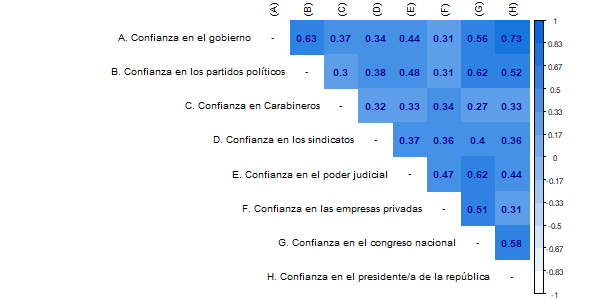
\includegraphics[width=1\linewidth,height=1\textheight]{output/graphs/confianza-institucional_cor} 

}

\caption{Asociación indicadores Confianza institucional.}\label{fig:confianza-institucional-cor}
\end{figure}

\hypertarget{orientaciuxf3n-hacia-el-bien-comuxfan}{%
\section{Orientación hacia el bien común}\label{orientaciuxf3n-hacia-el-bien-comuxfan}}

Esta tercera dimensión refiere a ``una actitud favorable a acciones que propendan a un mayor bienestar colectivo versus el beneficio puramente individual como parte de un proyecto compartido, o bien, como indican Sorj y Tironi (2007), aceptar ``vivir en un orden colectivo que les reportará beneficios, así como sacrificios individuales''." (CEPAL, \protect\hyperlink{ref-cepal_Cohesion_2021}{2021}, p. 46)

\textbf{Solidaridad}

La subdimensión de solidaridad busca cuantificar la presencia de valores solidarios en los individuos de la sociedad. Esta solidaridad se basa en el ``entendimiento de la reciprocidad aprendida en redes, y es un reflejo de la solidaridad que perciben recibir por parte del Estado y sus pares (CEPAL, 2007)'' (CEPAL, \protect\hyperlink{ref-cepal_Cohesion_2021}{2021}, p. 66).

En informe CEPAL utilizan el indicador ``Asistencia a reuniones de un grupo de mejoras para la comunidad'', que cuantifica la asistencia a reuniones para mejorar su comunidad. Al trabajar con ELSOC se utilizará este indicador y otros siete que abordan un comportamiento prosocial y que están presentes en las cuatro olas. Un análisis descriptivo de estos indicadores se presentan en la Figura \ref{fig:solidaridad} y un análisis bivariado en la Figura \ref{fig:solidaridad-cor}.

\begin{figure}[H]

{\centering 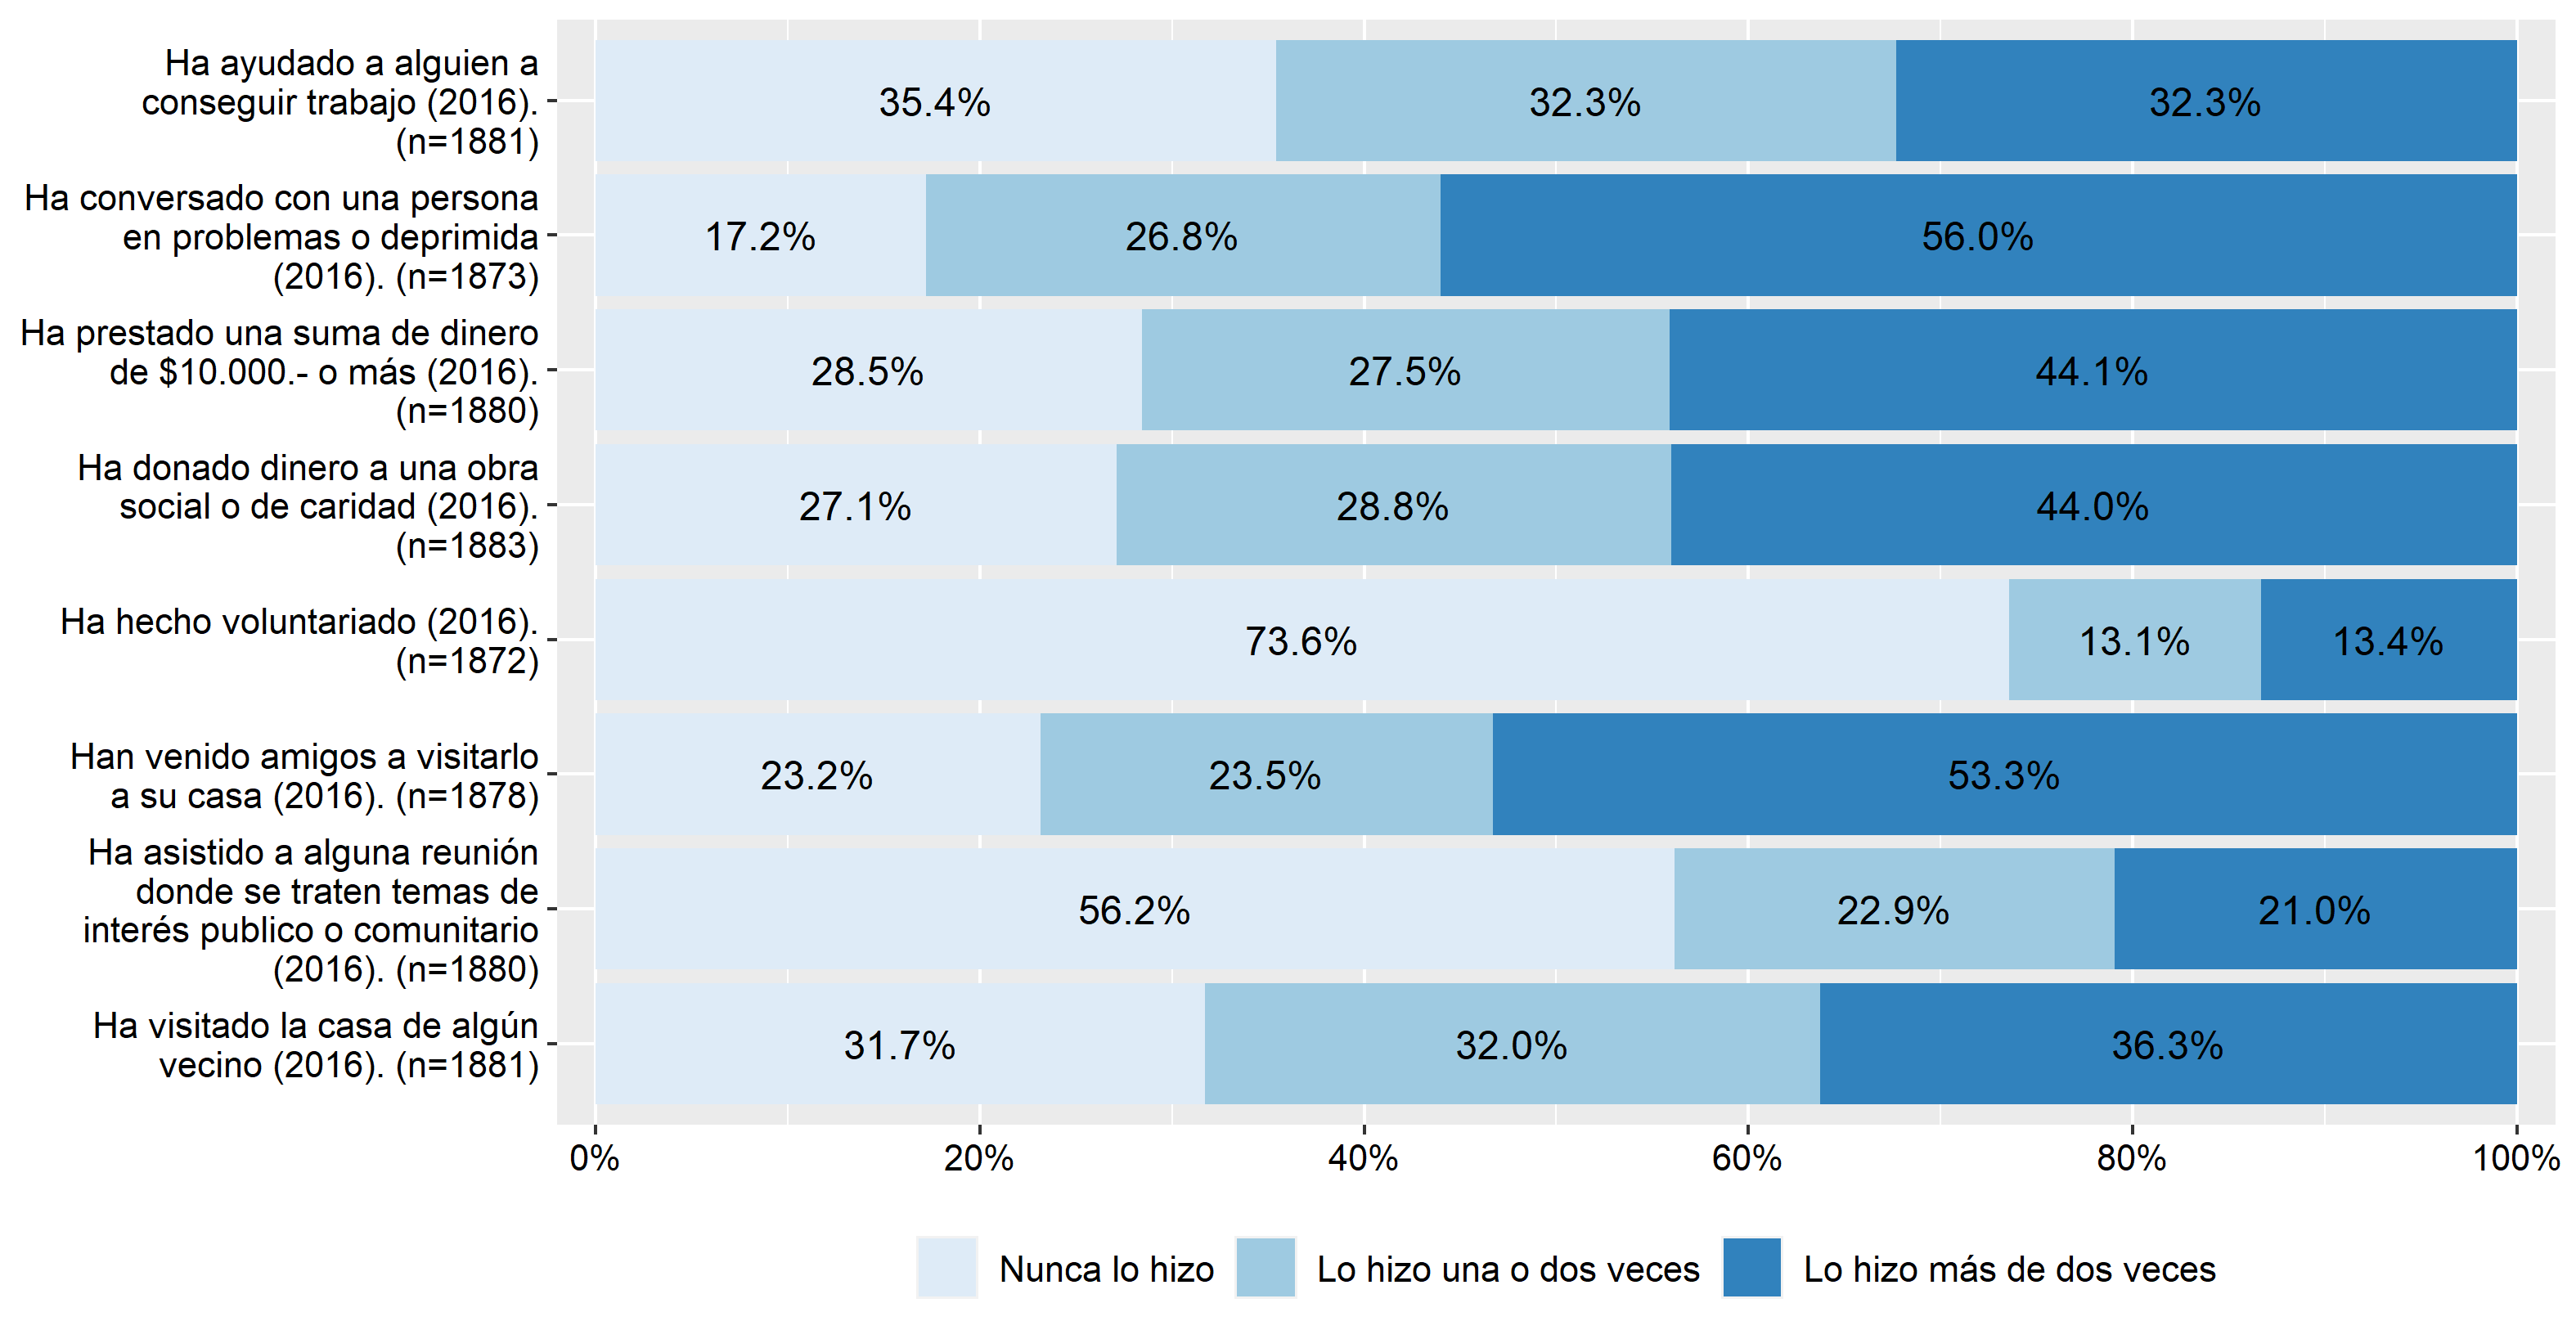
\includegraphics[width=1\linewidth,height=1\textheight]{output/graphs/solidaridad} 

}

\caption{Acciones de solidaridad.}\label{fig:solidaridad}
\end{figure}

\begin{figure}[H]

{\centering 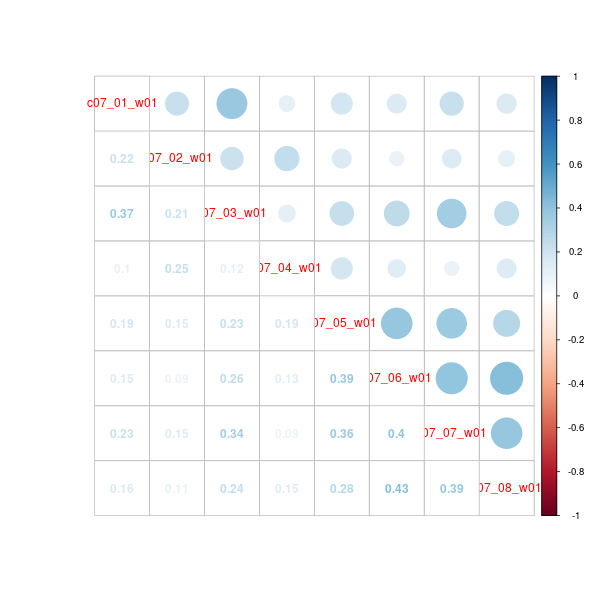
\includegraphics[width=1\linewidth,height=1\textheight]{output/graphs/solidaridad_cor} 

}

\caption{Asociación indicadores de solidaridad.}\label{fig:solidaridad-cor}
\end{figure}

\textbf{Participación cívica}

La subdimensión de participación cívica da cuenta de la voluntad de adherir a los espacios de participación del sistema político y la vinculación de los individuos con su comunidad. Esta participación ``promueve la participación ciudadana en los asuntos públcios, apoyando pryectos colectivas que representen sus opiniones o intereses políticos (Valdéz, Viramontes y Finol, 2016)'' (CEPAL, \protect\hyperlink{ref-cepal_Cohesion_2021}{2021}, p. 66).

En informe CEPAL se utilizaron los indicadores ``Tiene actividad política (firma peticiones, boicot, va a manifestaciones pacíficas, huelgas)'', que indica la predisposición hacia la actividad política, ``Participación en organizaciones'', que busca medir la implicación de los individuos con su comunidad y ``Voto en elecciones presidenciales'', que pretende capturar el grado de compromiso cívico con el sistema regente y la dirección de la sociedad. Al trabajar con ELSOC se utilizan cuatro indicadores de actividad política presentes en las cuatro olas, ocho indicadores de participación en organizaciones presentes en ola 1 y 3 y voto en elecciones 2013 y 2017 (ola 1 y 3). Un análisis descriptivo de estos indicadores se presentan en la Figura \ref{fig:participacion-civica}, en la Figura \ref{fig:participacion-organizaciones} y en la Figura \ref{fig:participacion-electoral}, mientras que un análisis bivariado en la Figura \ref{fig:participacion-civica-cor} y en la Figura \ref{fig:participacion-organizaciones-cor}.

\begin{figure}[H]

{\centering 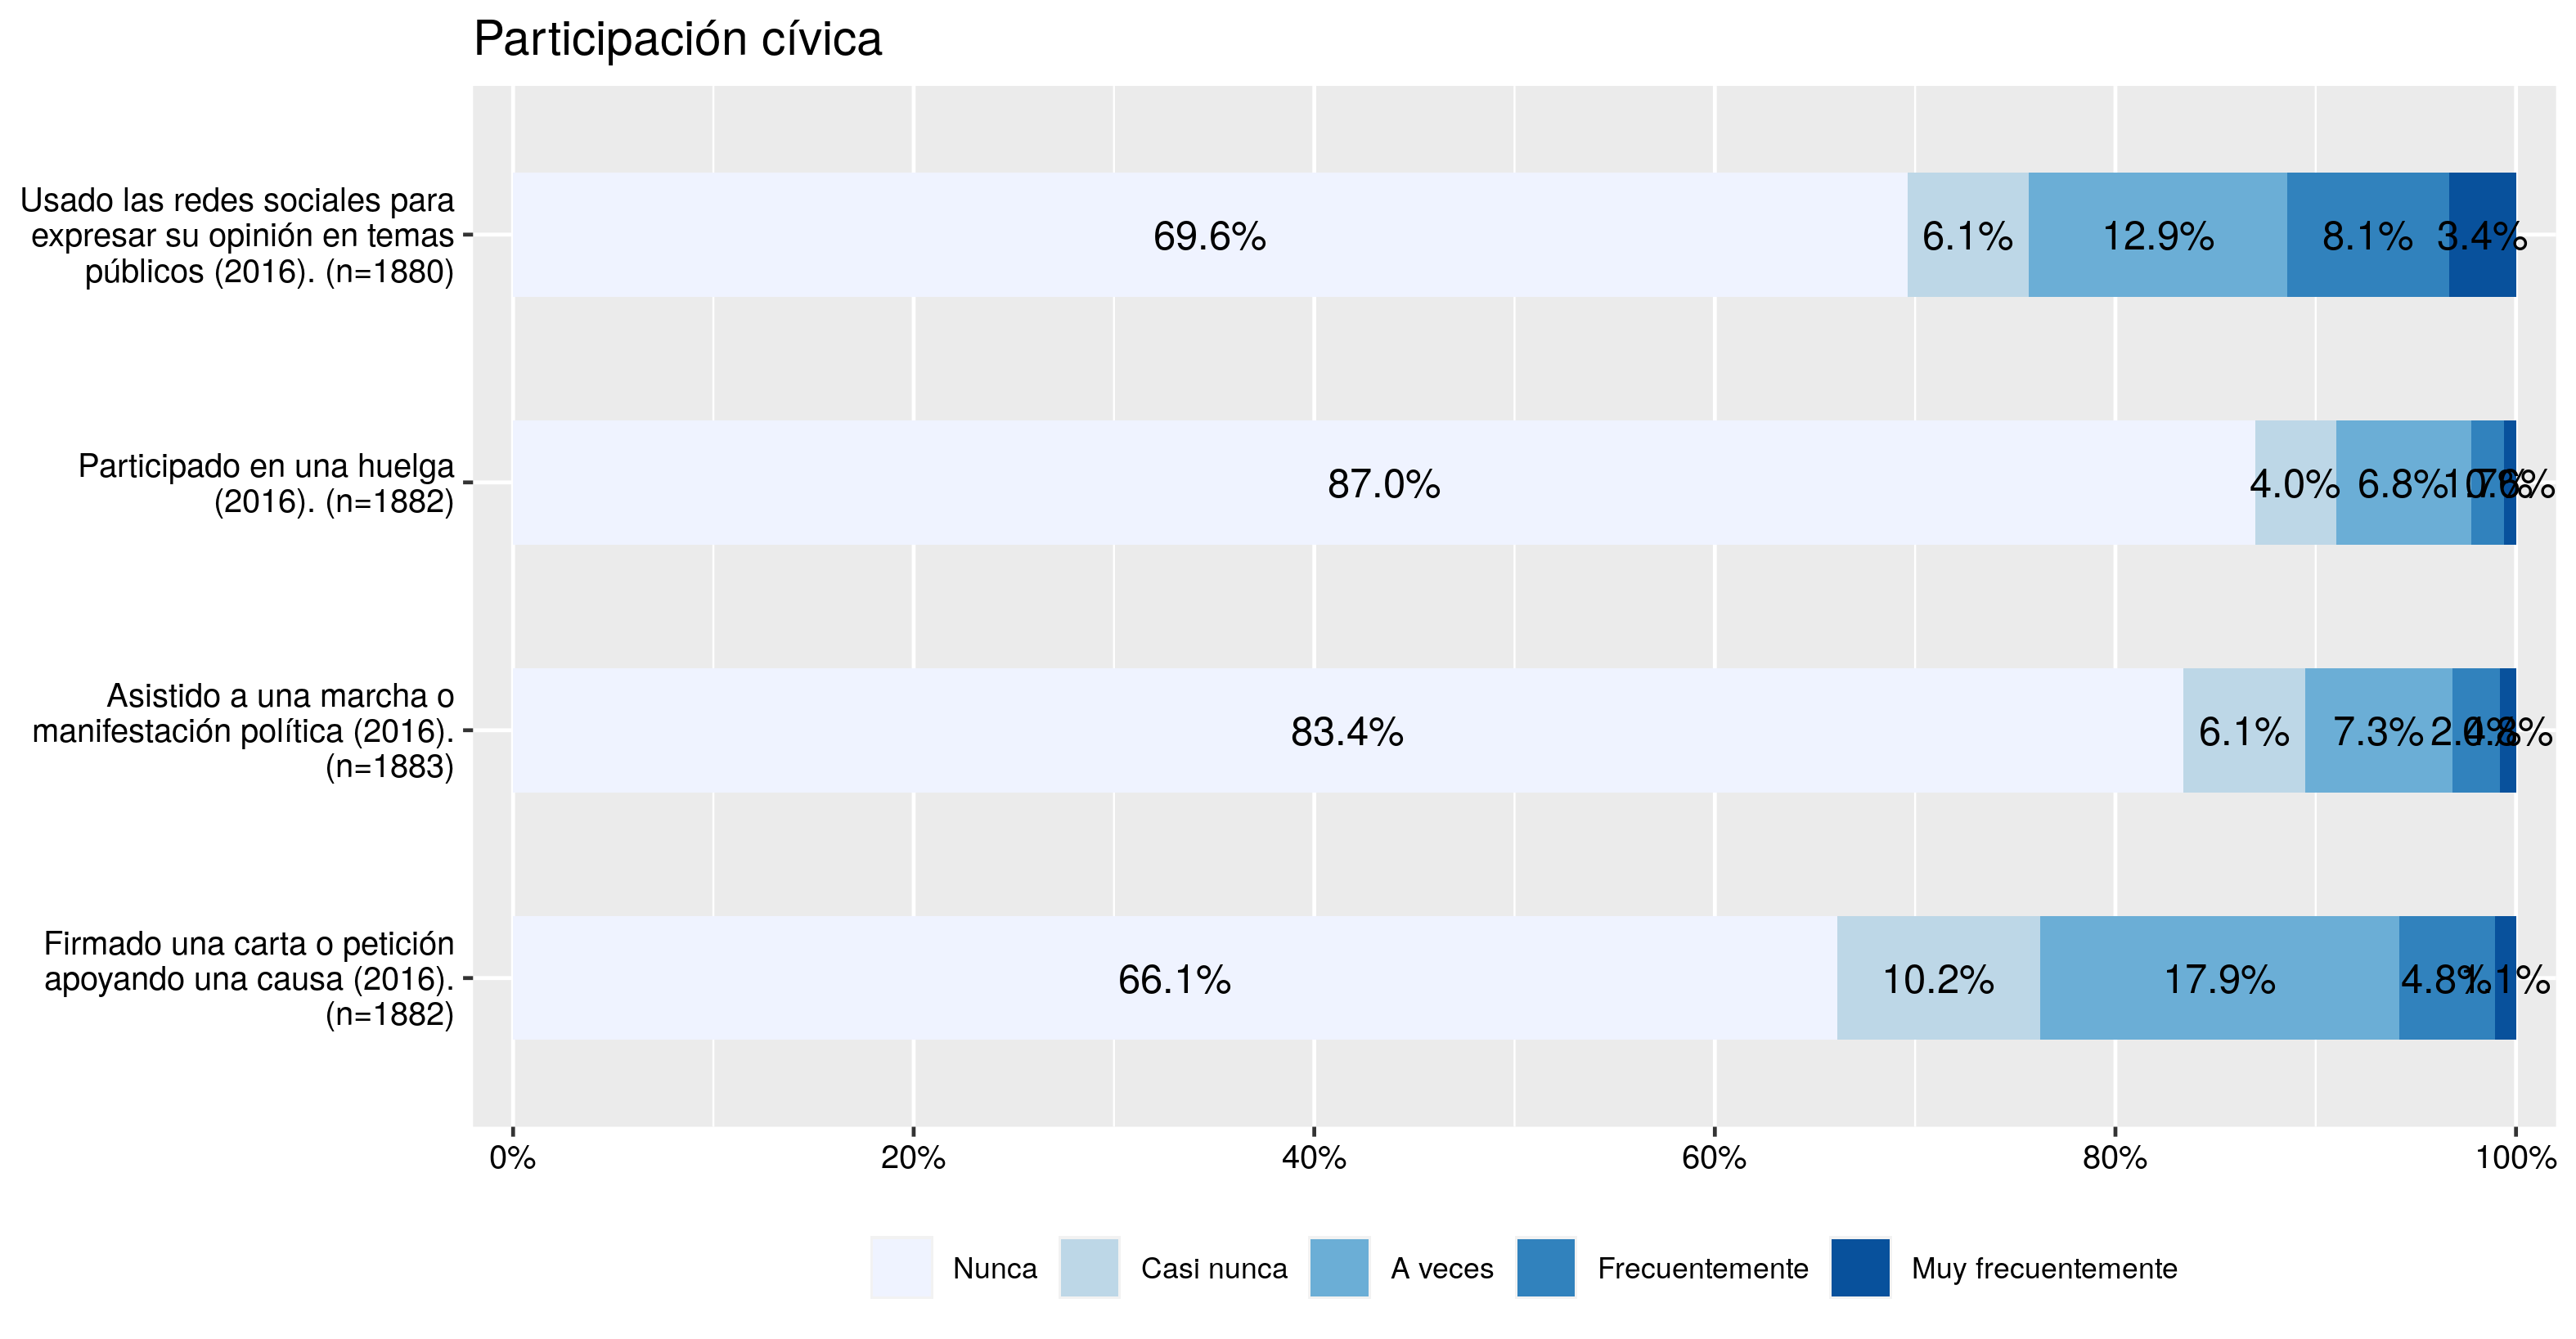
\includegraphics[width=1\linewidth,height=1\textheight]{output/graphs/participacion-civica} 

}

\caption{Participación en actividades cívicas.}\label{fig:participacion-civica}
\end{figure}

\begin{figure}[H]

{\centering 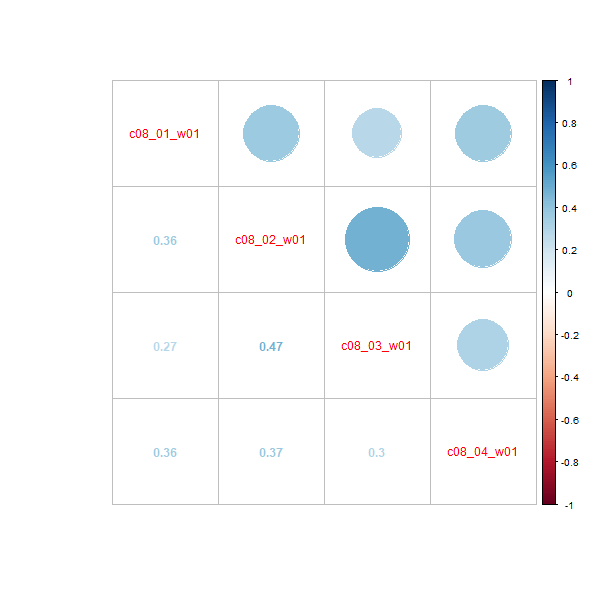
\includegraphics[width=1\linewidth,height=1\textheight]{output/graphs/participacion-civica_cor} 

}

\caption{Asociación indicadores participación cívica.}\label{fig:participacion-civica-cor}
\end{figure}

\textbf{Participación en organizaciones}

\begin{figure}[H]

{\centering 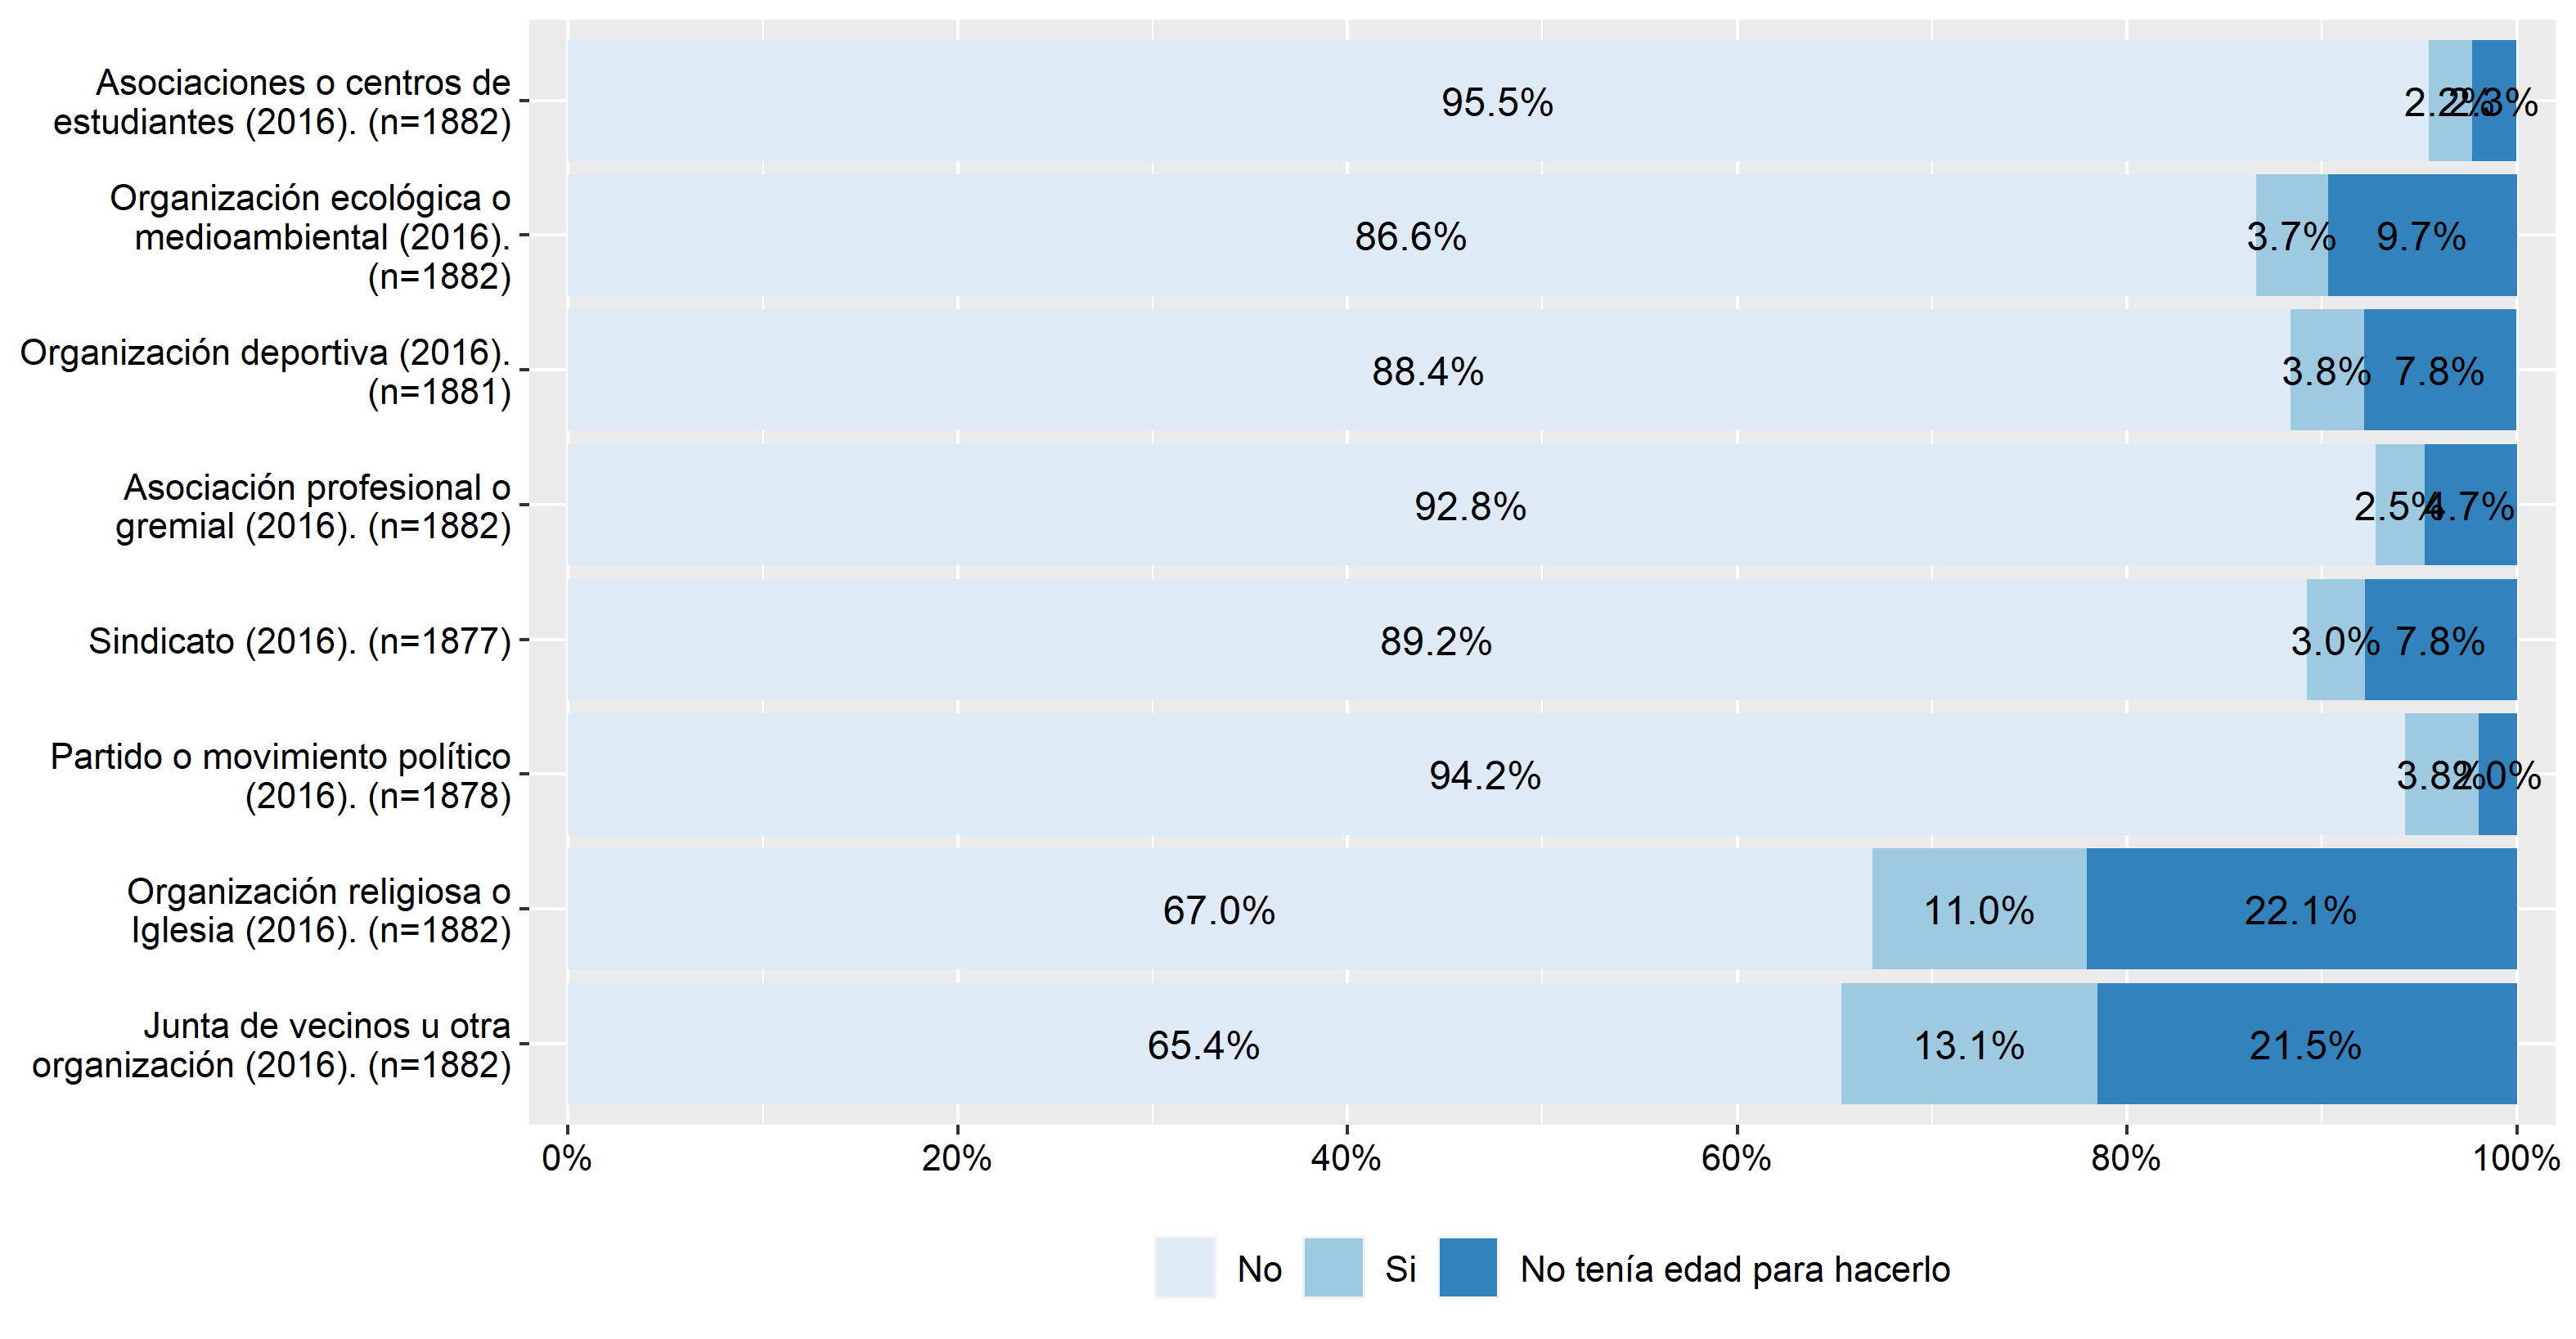
\includegraphics[width=1\linewidth,height=1\textheight]{output/graphs/participacion-organizaciones} 

}

\caption{Participación en organizaciones sociales.}\label{fig:participacion-organizaciones}
\end{figure}

\begin{figure}[H]

{\centering 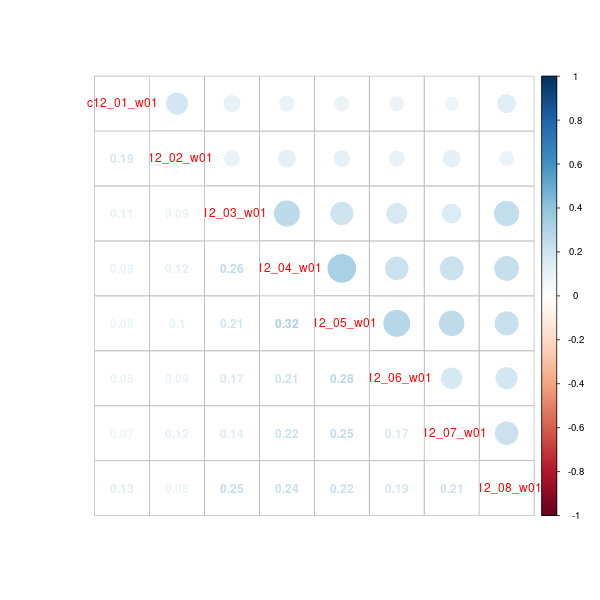
\includegraphics[width=1\linewidth,height=1\textheight]{output/graphs/participacion-organizaciones_cor} 

}

\caption{Asociación indicadores participación en organizaciones.}\label{fig:participacion-organizaciones-cor}
\end{figure}

\textbf{Participación electoral}

\begin{figure}[H]

{\centering 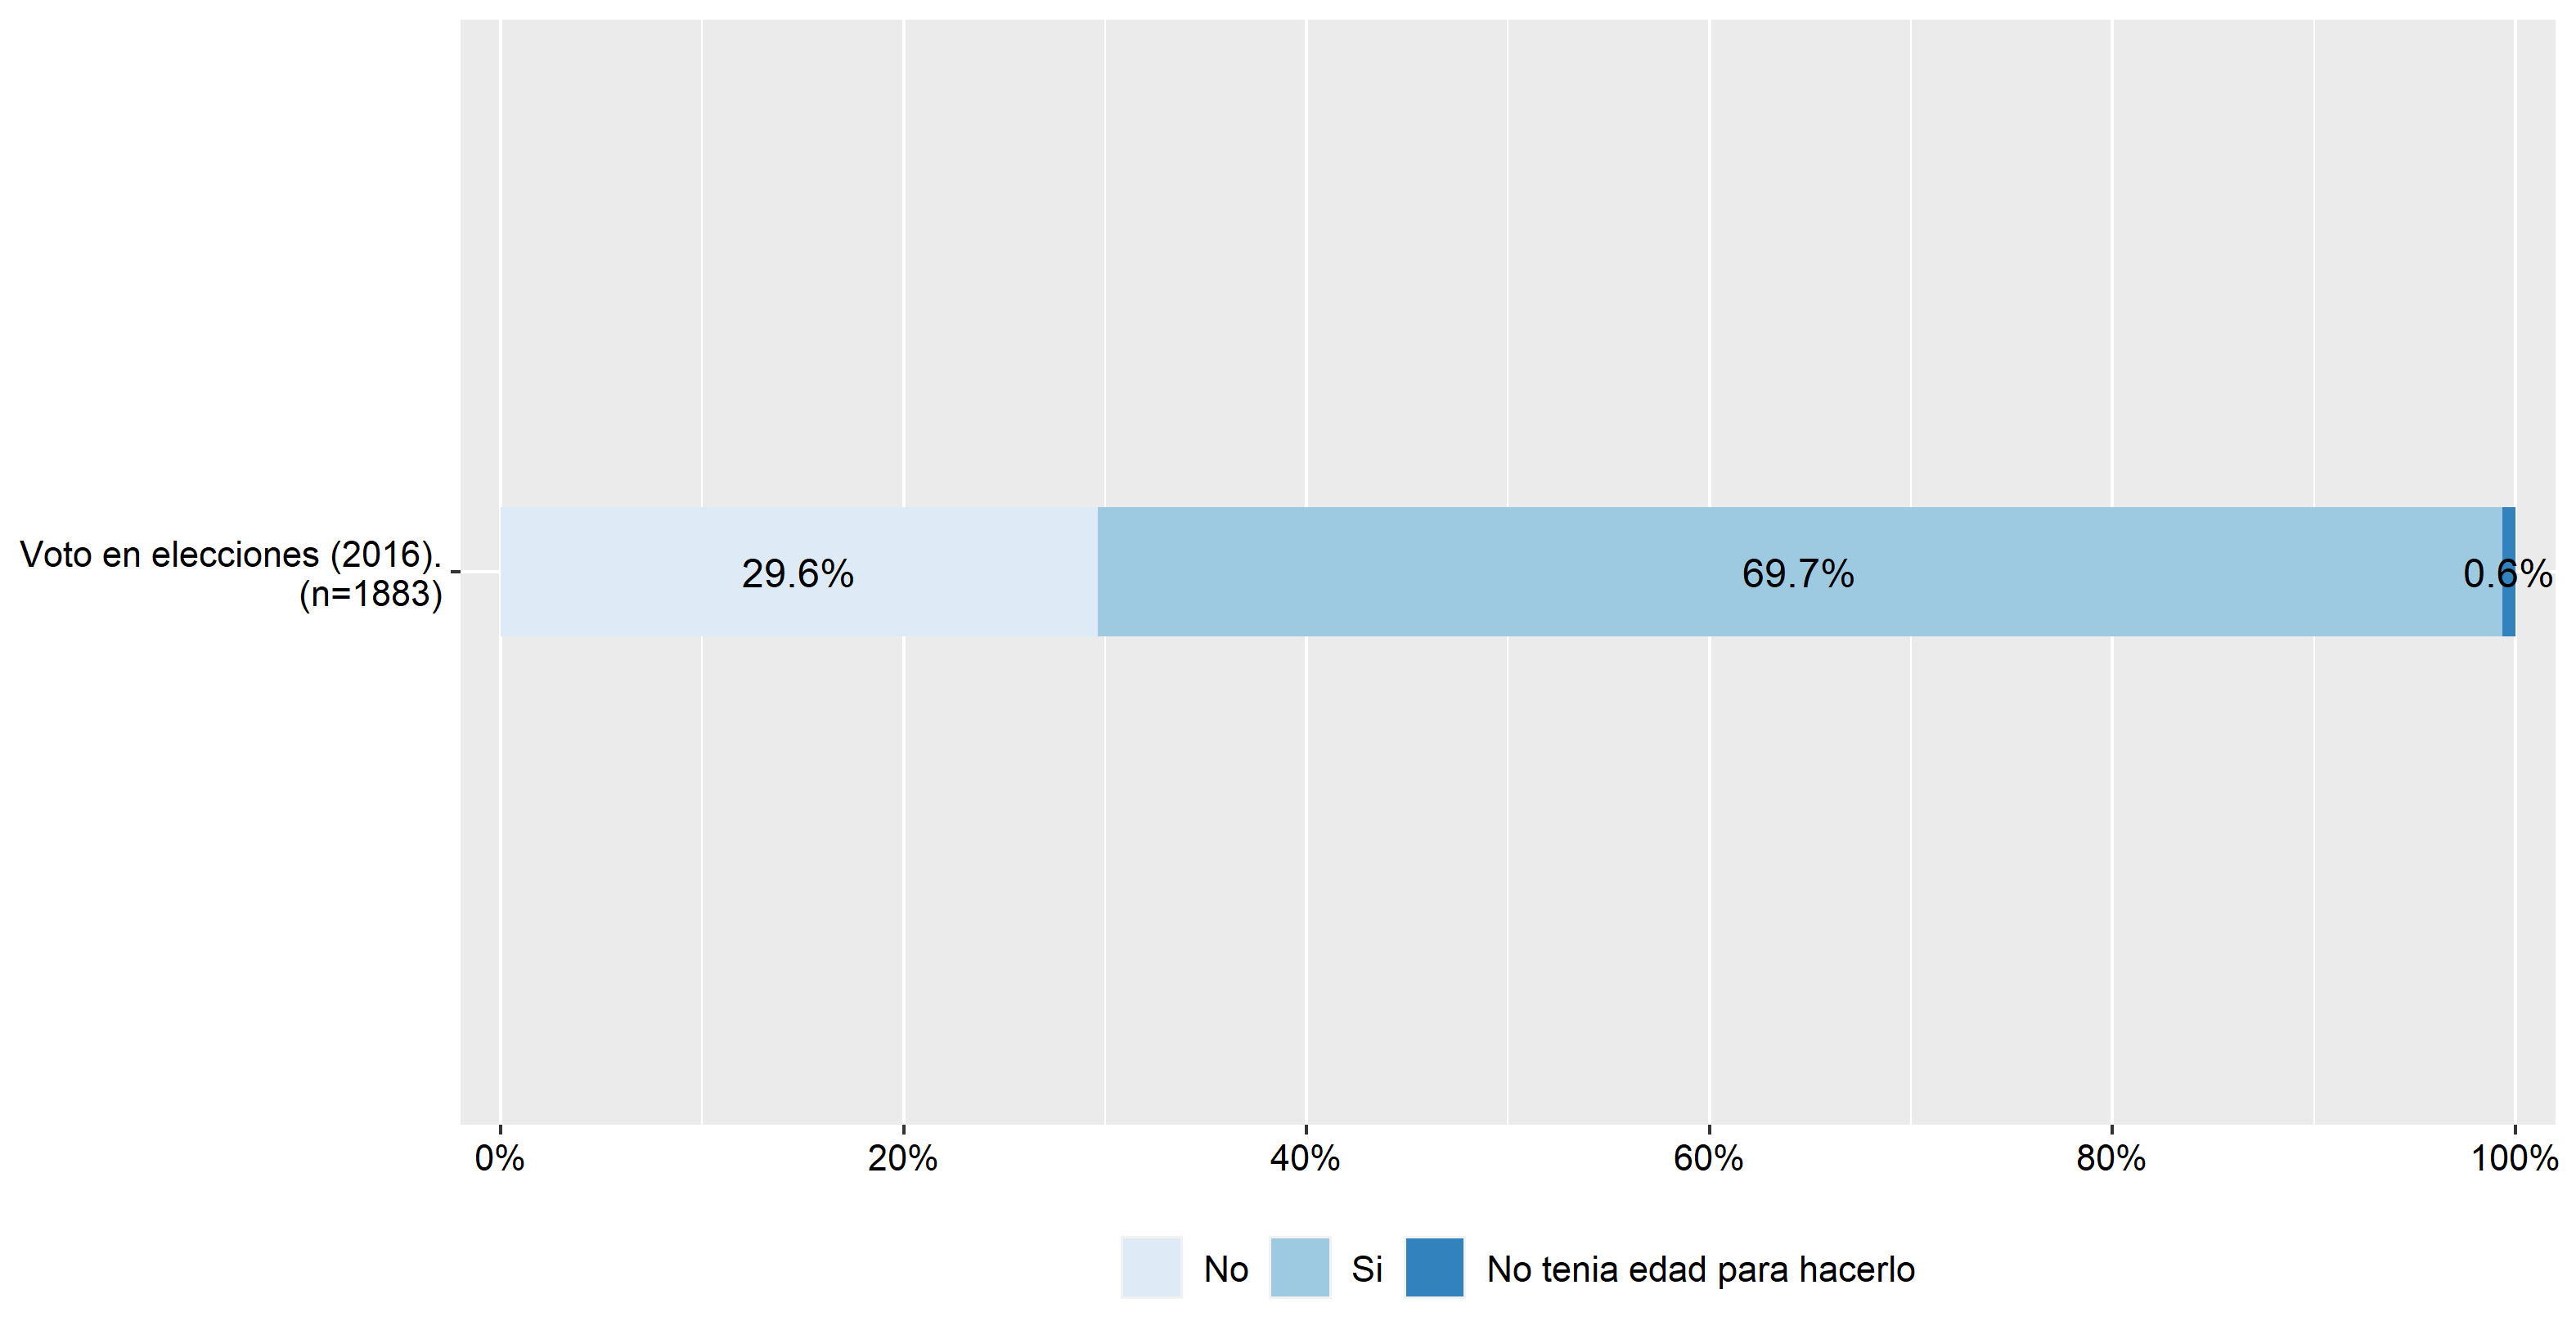
\includegraphics[width=1\linewidth,height=1\textheight]{output/graphs/participacion-electoral} 

}

\caption{Participación en elecciones 2013 y 2017.}\label{fig:participacion-electoral}
\end{figure}

\hypertarget{cohesiuxf3n-territorial}{%
\section{Cohesión territorial}\label{cohesiuxf3n-territorial}}

De manera adicional, se incorpora una dimensión sobre calidad de vida en el vecindario presente en ELSOC. Todos estos indicadores se encuentran presentes en las cuatro olas.

\textbf{Confianza en vecinos}

\begin{figure}[H]

{\centering 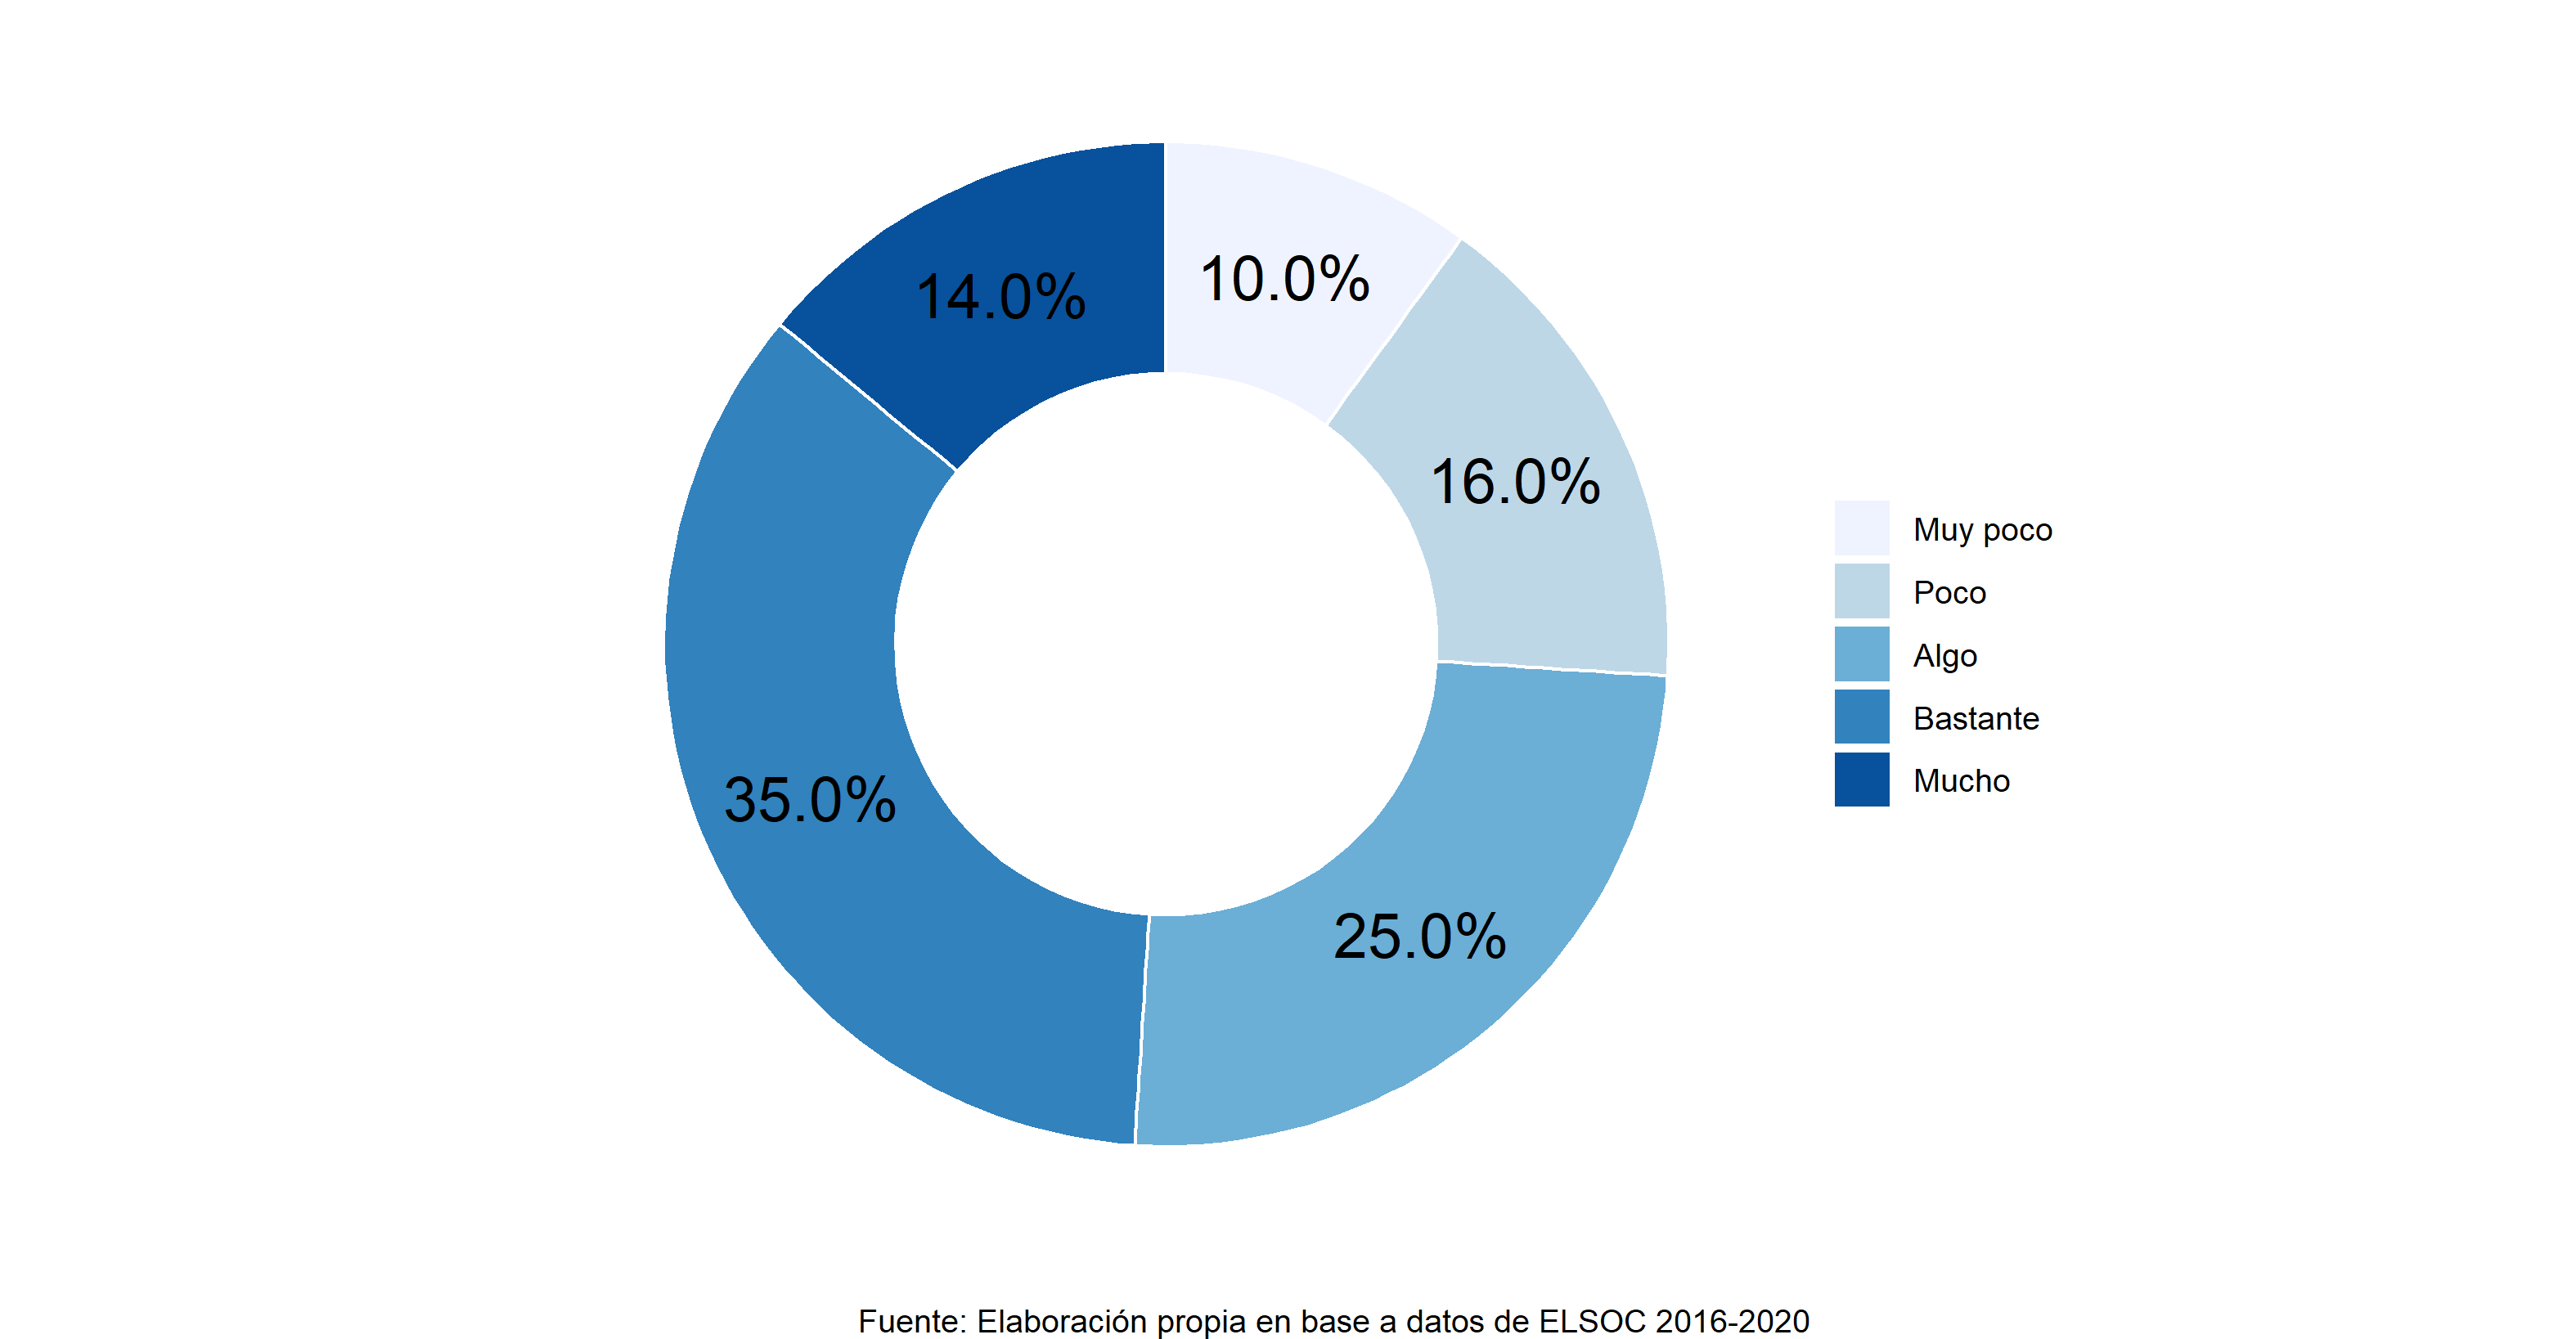
\includegraphics[width=1\linewidth,height=1\textheight]{output/graphs/confianza-vecinos} 

}

\caption{Confianza en vecinos.}\label{fig:unnamed-chunk-3}
\end{figure}

\textbf{Identificación barrial}

\begin{figure}[H]

{\centering 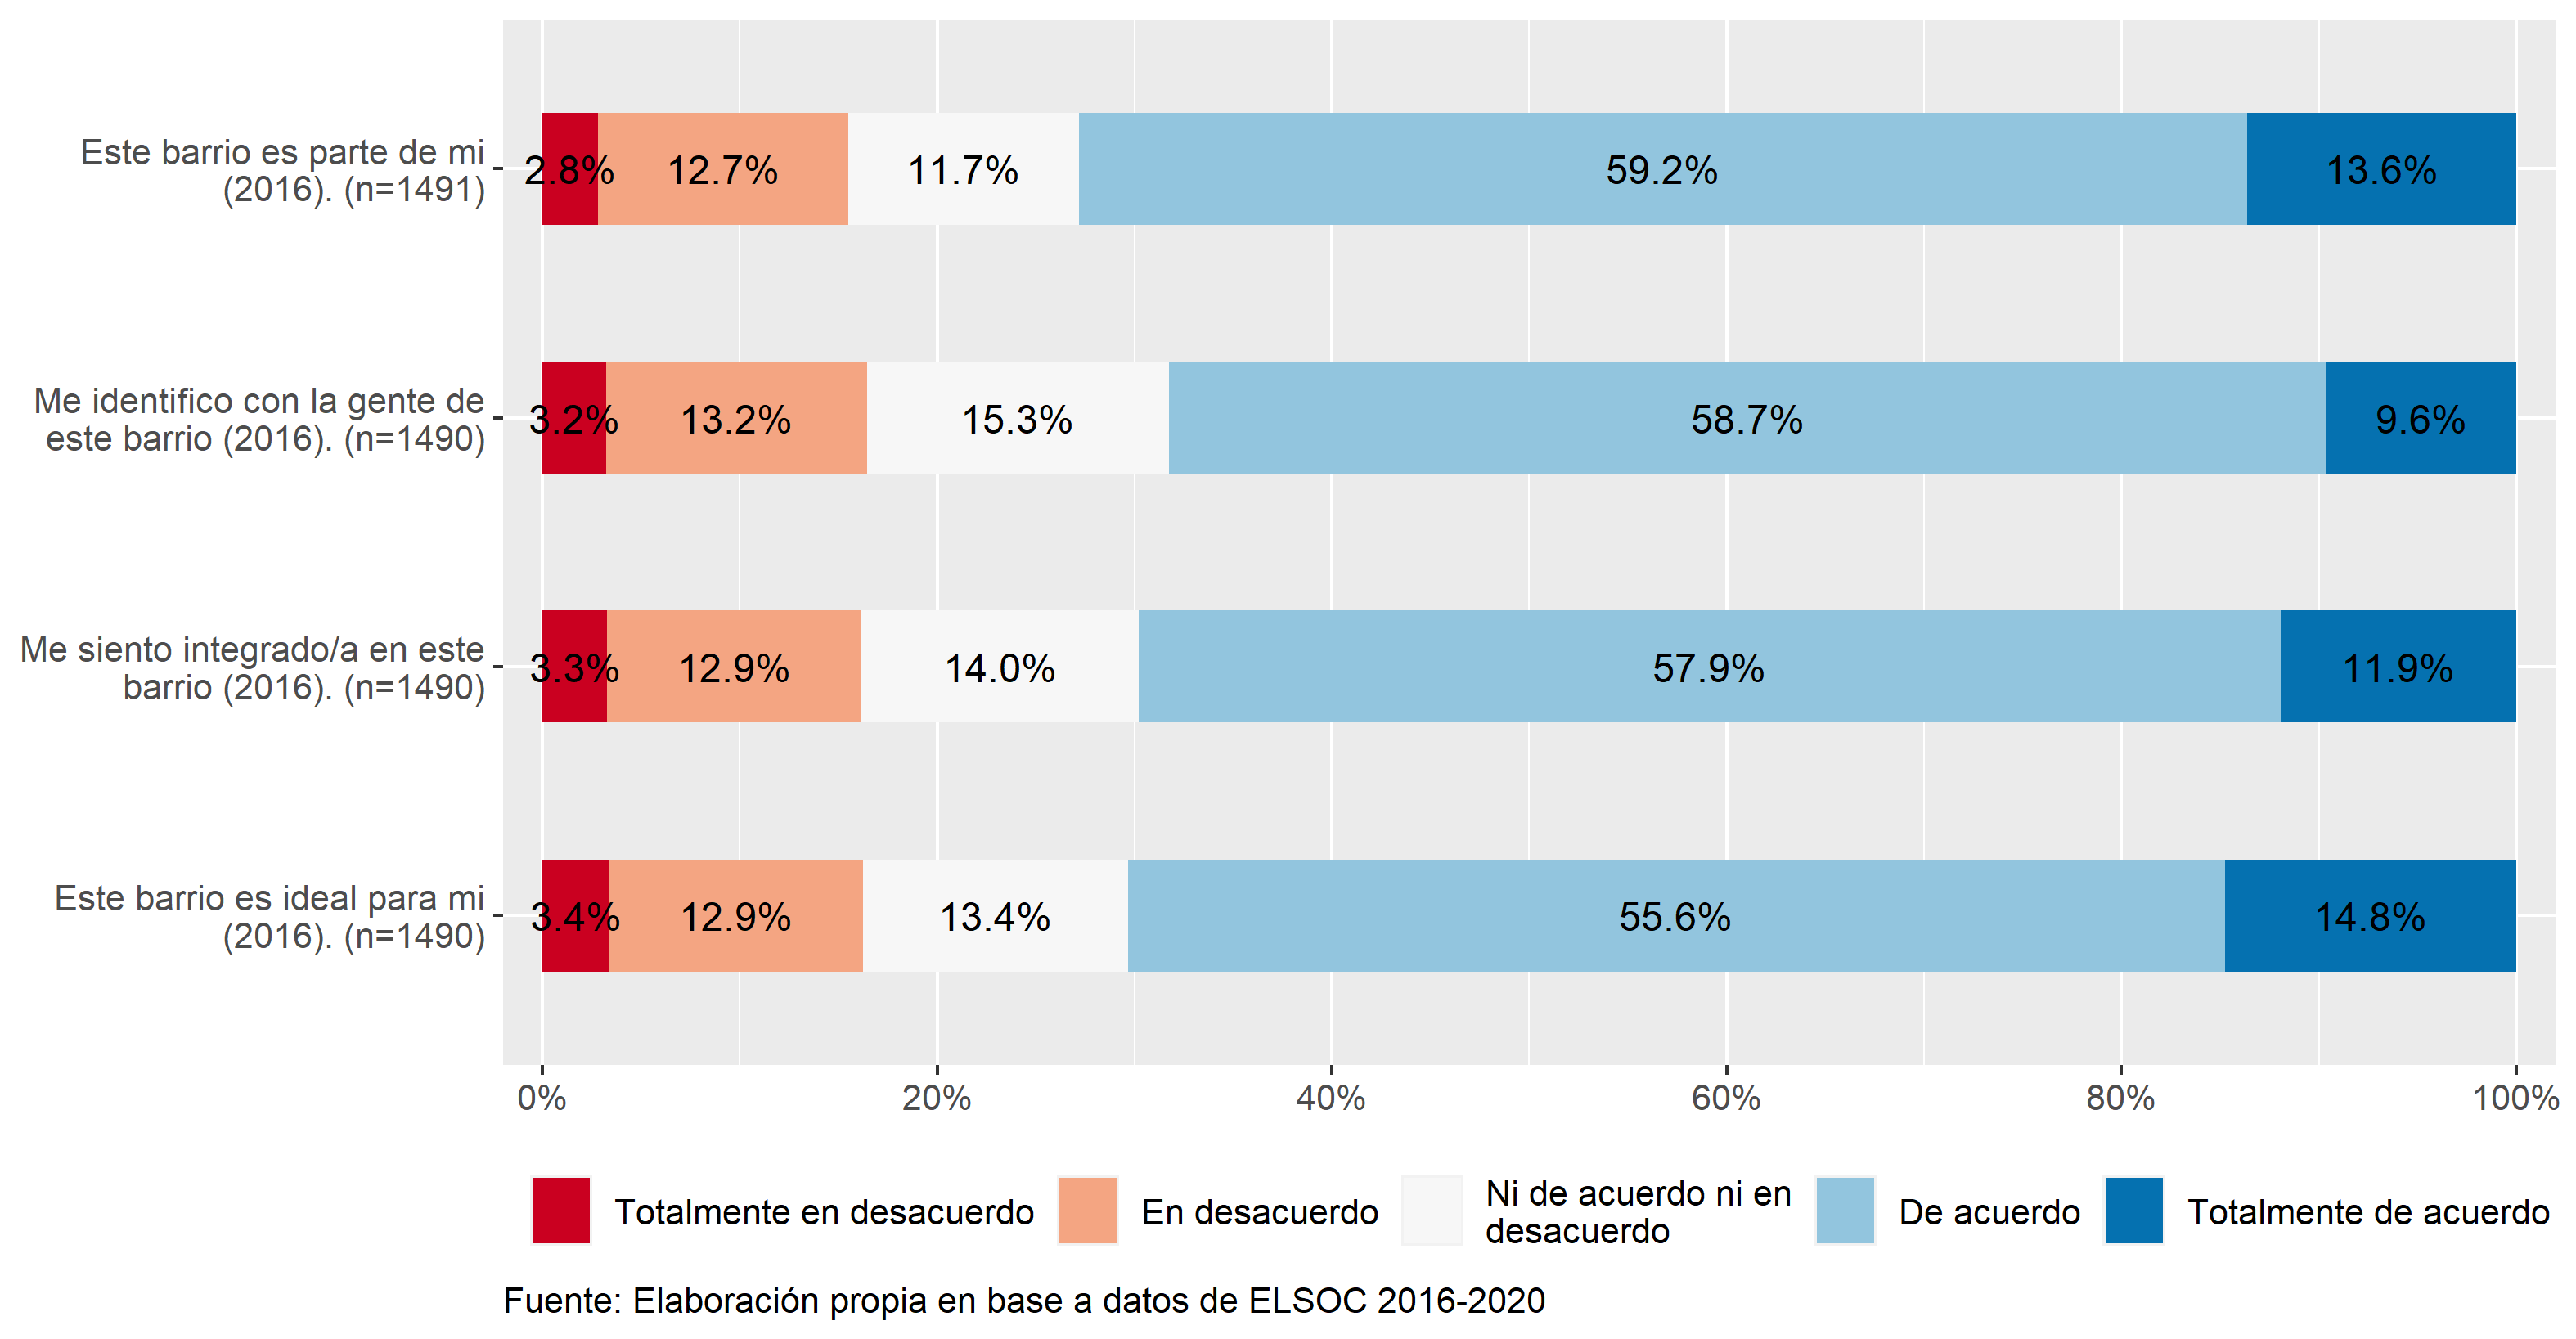
\includegraphics[width=1\linewidth,height=1\textheight]{output/graphs/cohesion-barrial} 

}

\caption{ Identificación con el barrio.}\label{fig:unnamed-chunk-4}
\end{figure}

\begin{figure}[H]

{\centering 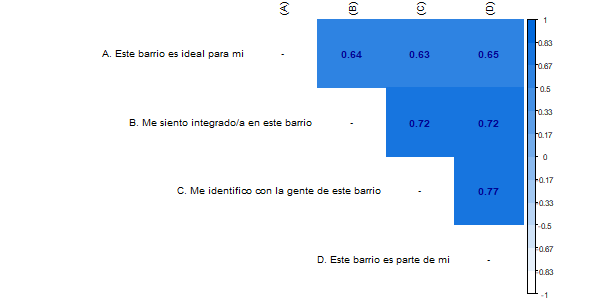
\includegraphics[width=1\linewidth,height=1\textheight]{output/graphs/cohesion-barrial_cor} 

}

\caption{Asociación indicadores identificación barrial.}\label{fig:unnamed-chunk-5}
\end{figure}

\textbf{Sociabilidad barrial}

\begin{figure}[H]

{\centering 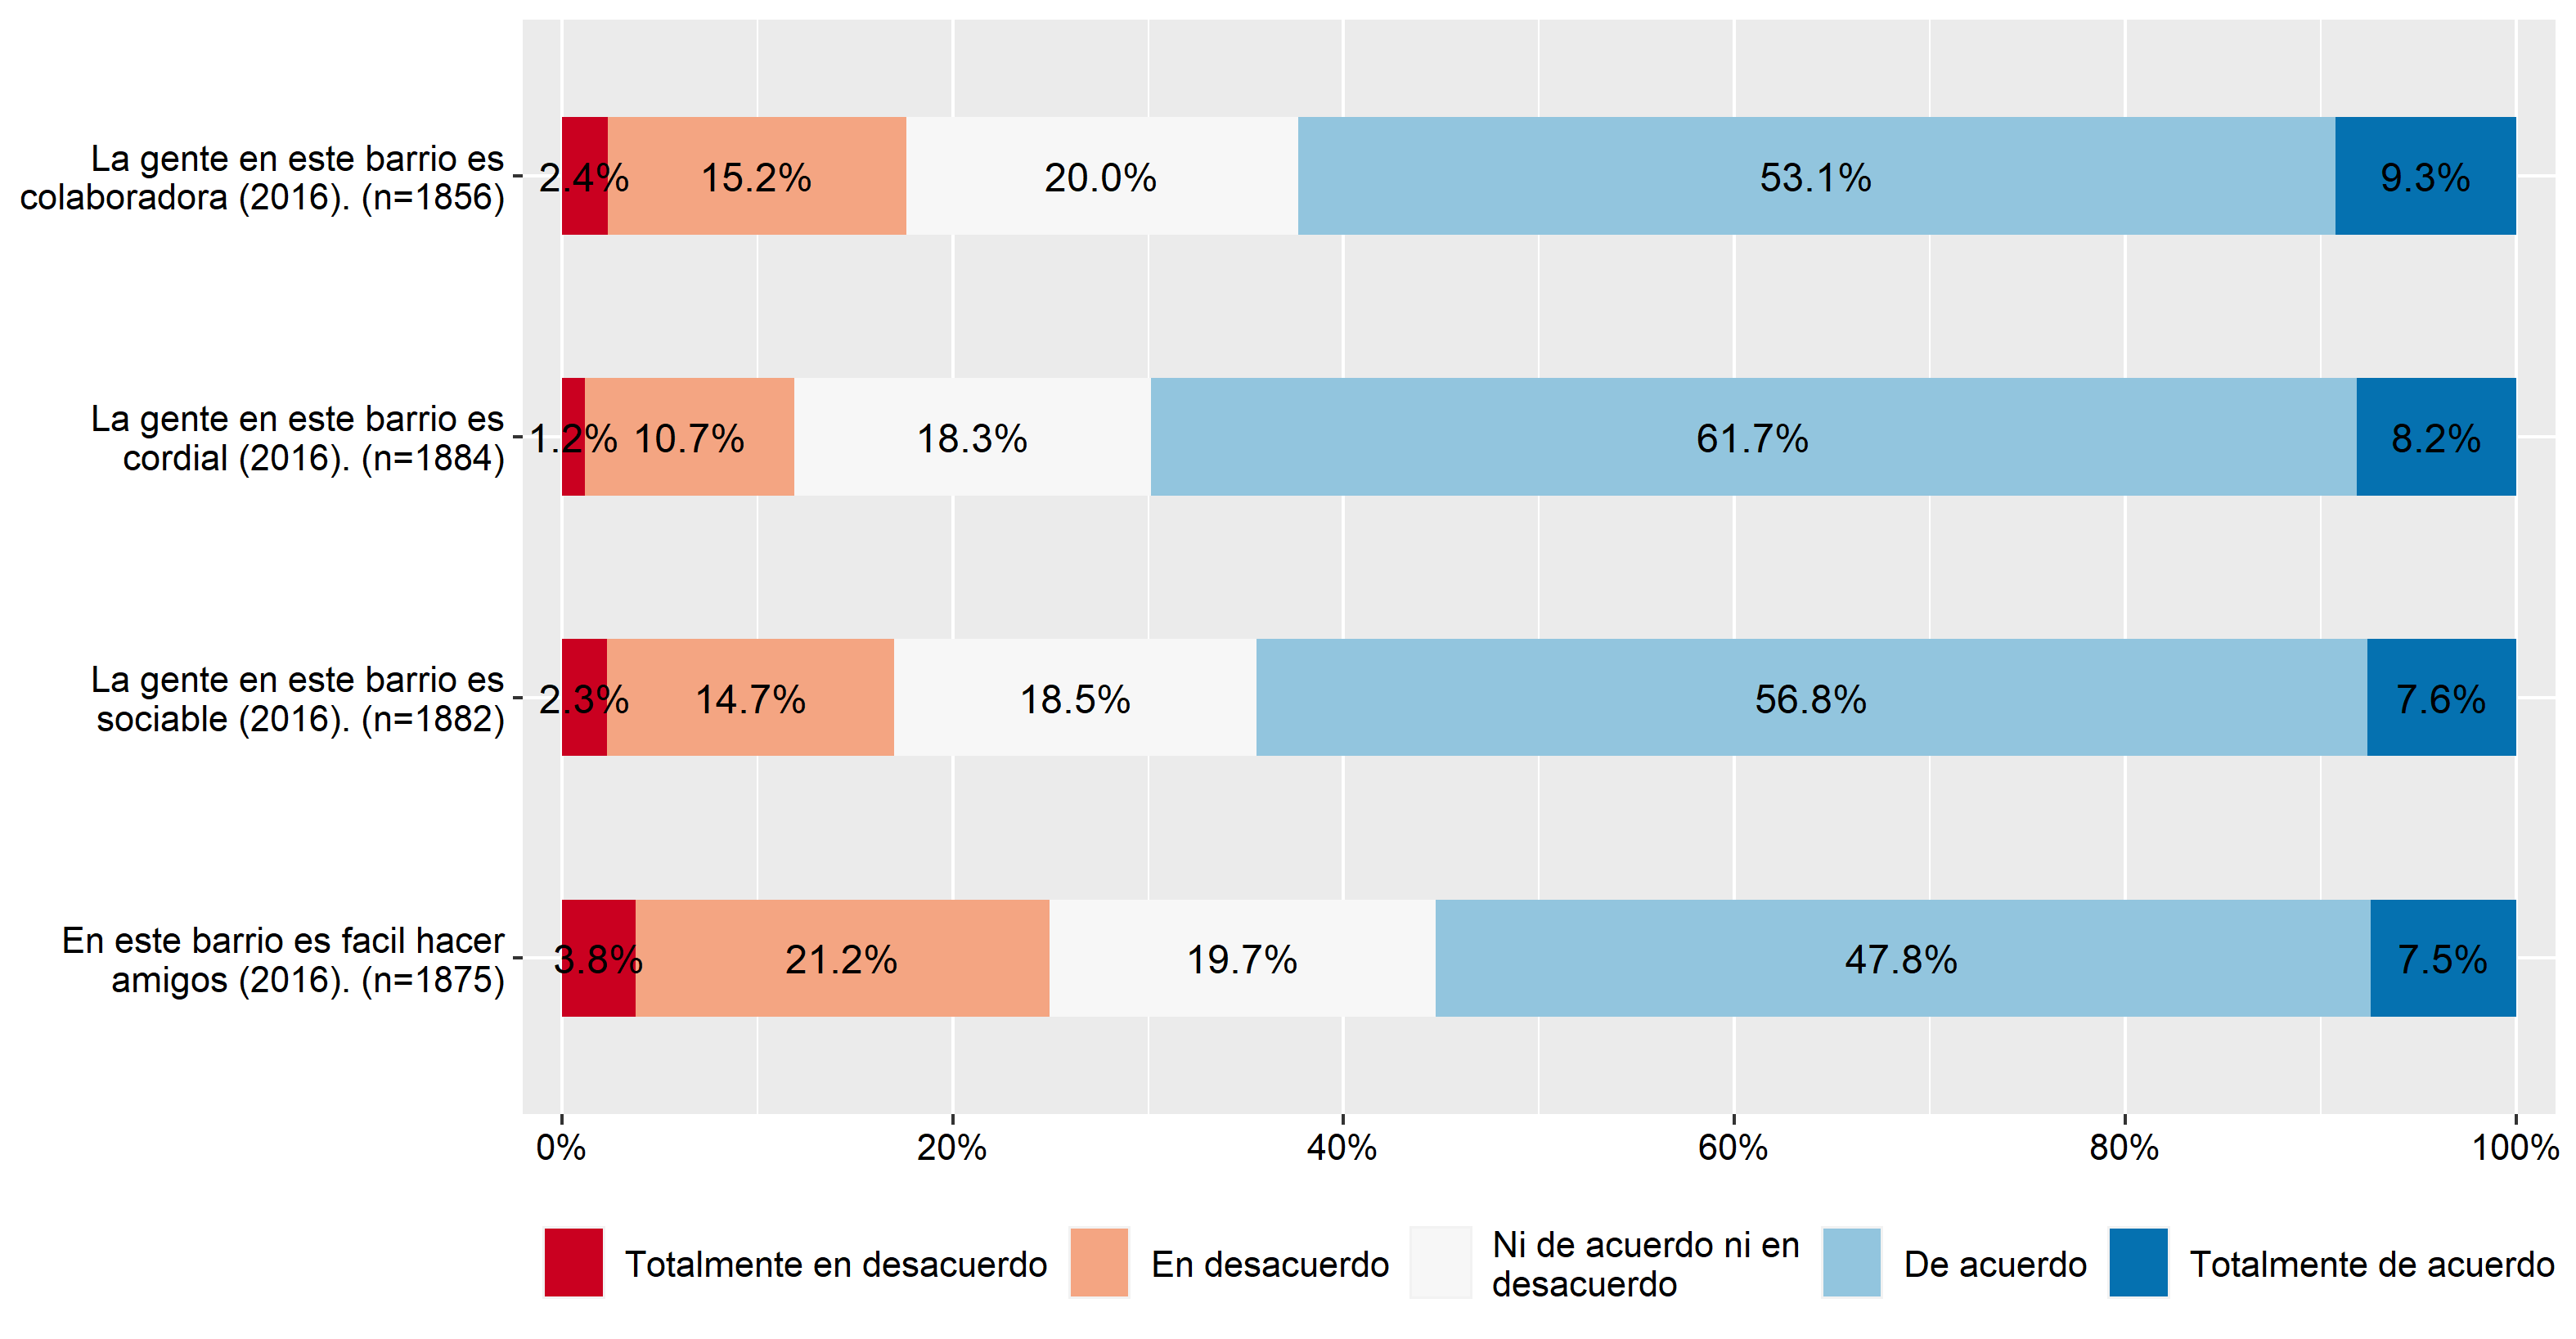
\includegraphics[width=1\linewidth,height=1\textheight]{output/graphs/sociabilidad-barrial} 

}

\caption{Sociabilidad barrial.}\label{fig:unnamed-chunk-6}
\end{figure}

\begin{figure}[H]

{\centering 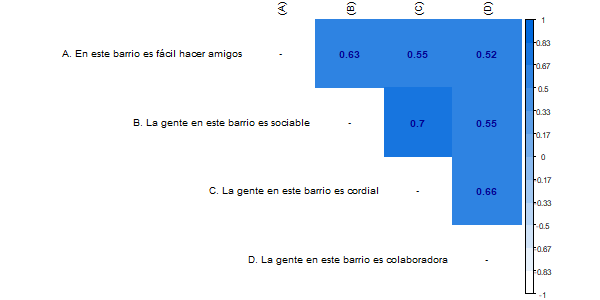
\includegraphics[width=1\linewidth,height=1\textheight]{output/graphs/sociabilidad-barrial_cor} 

}

\caption{Asociación indicadores sociabilidad barrial.}\label{fig:unnamed-chunk-7}
\end{figure}

\textbf{Satisfacción residencial}

\begin{figure}[H]

{\centering 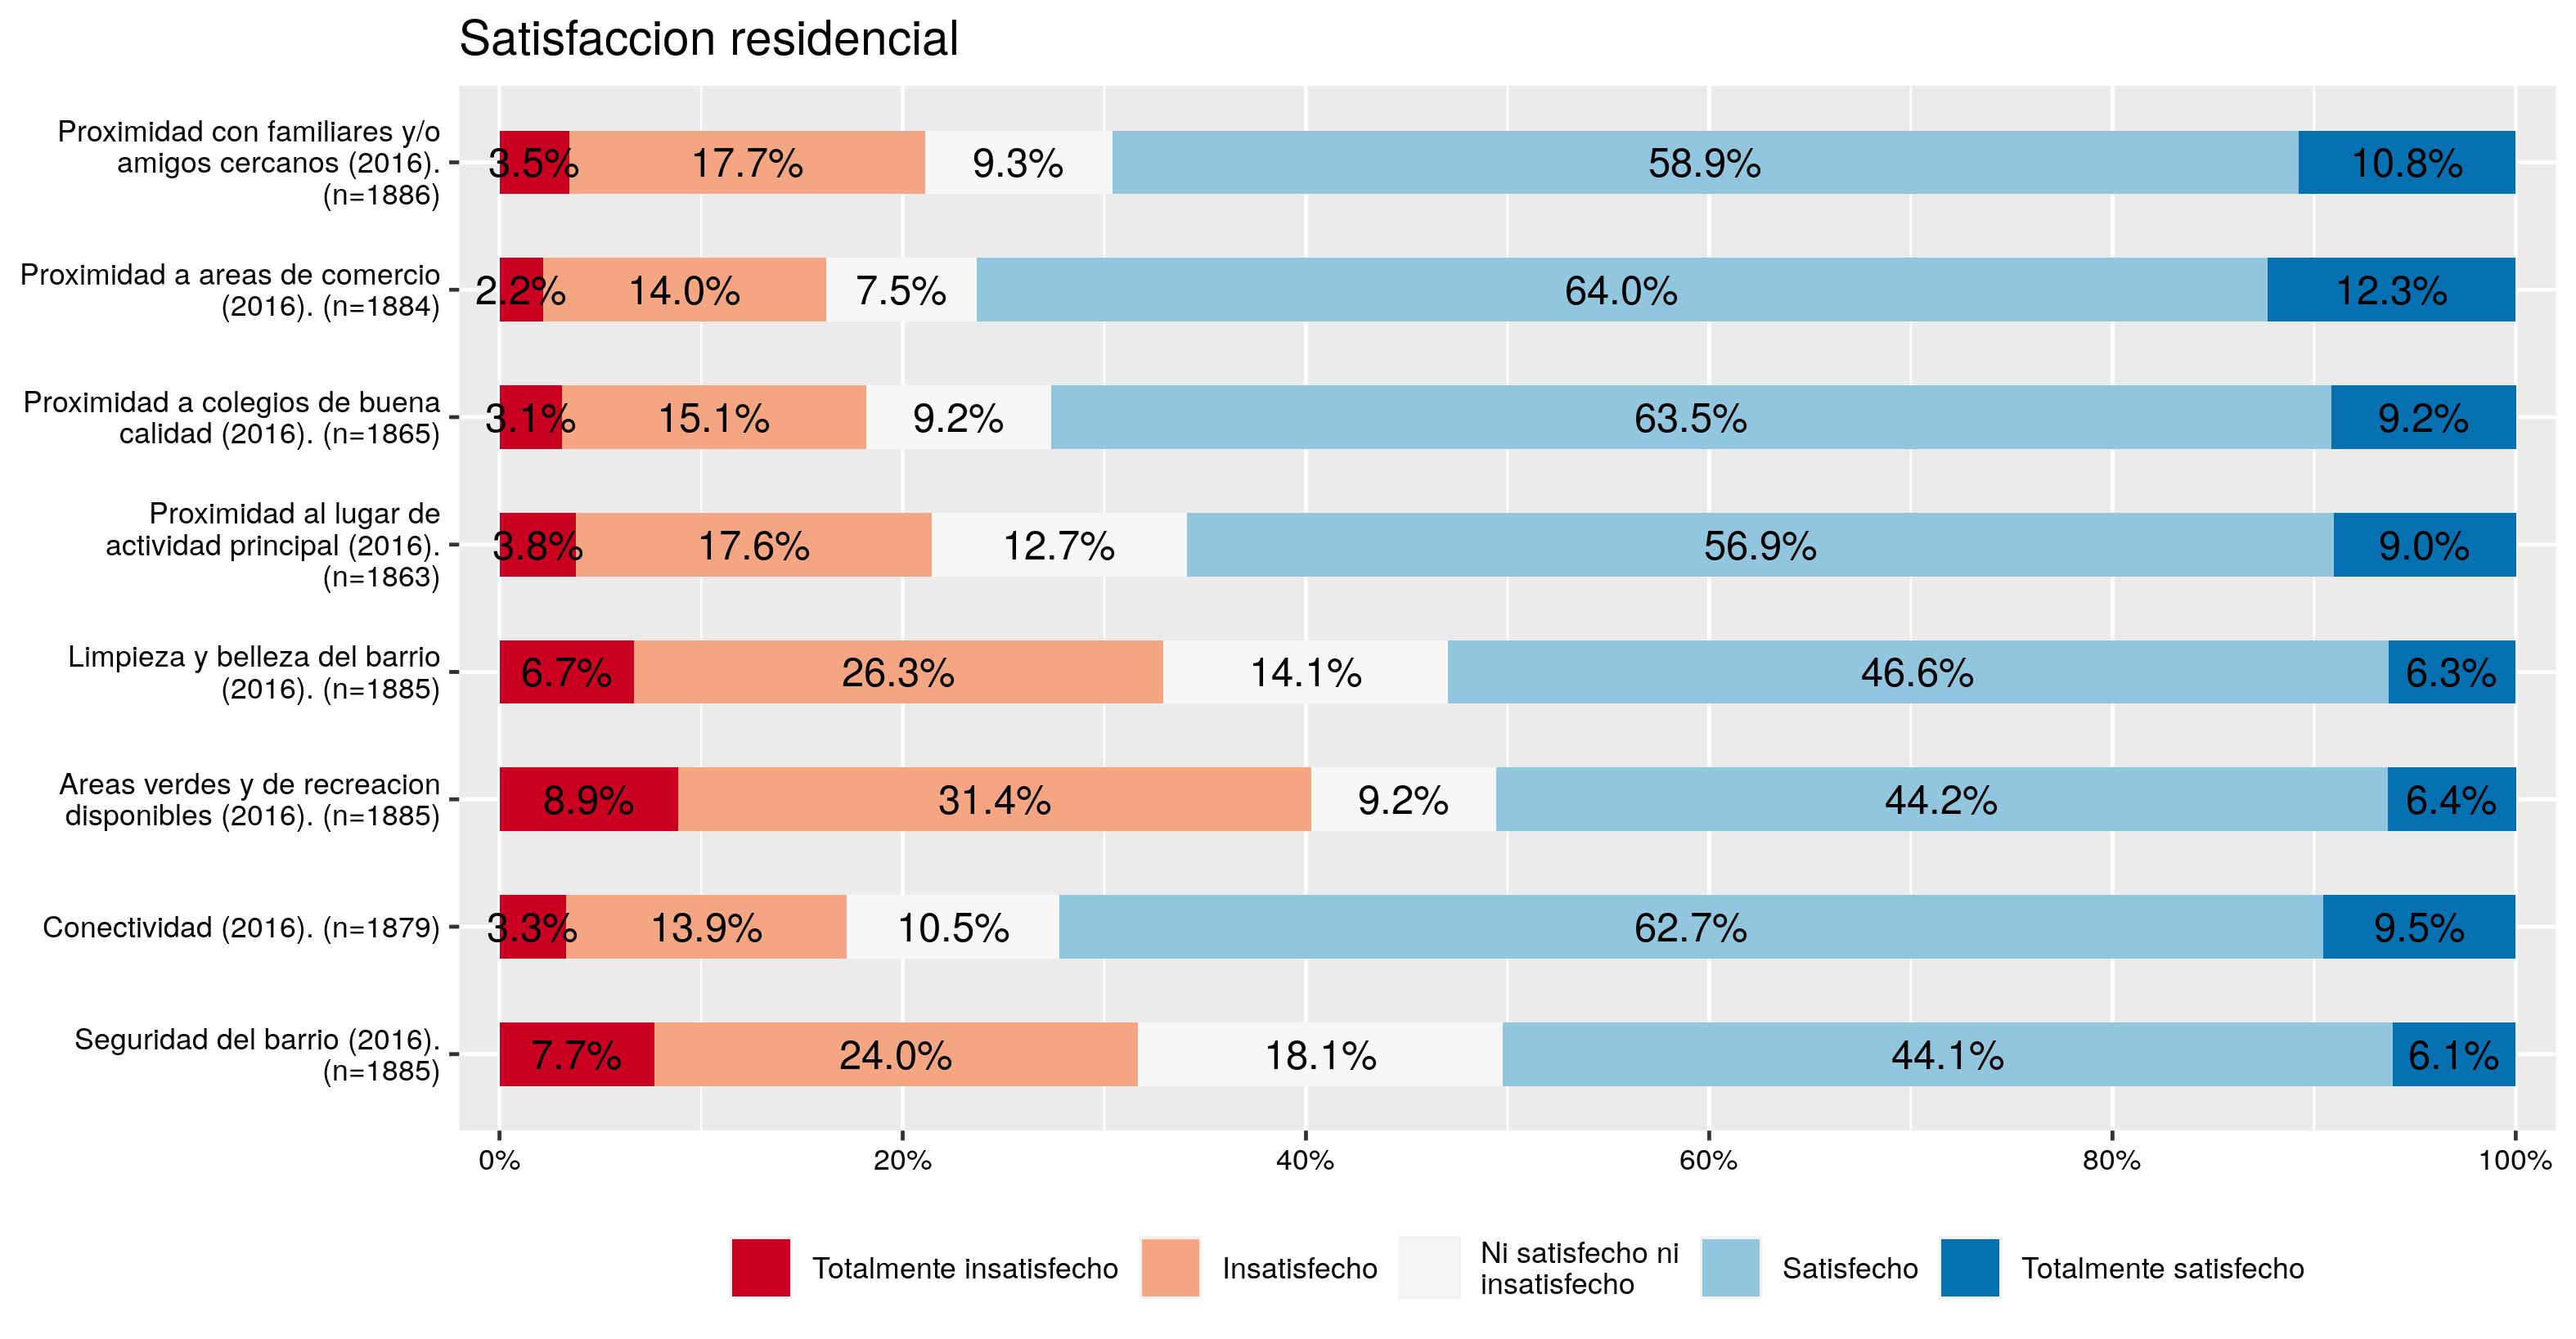
\includegraphics[width=1\linewidth,height=1\textheight]{output/graphs/satisfaccion-residencial} 

}

\caption{Satisfacción con el barrio.}\label{fig:unnamed-chunk-8}
\end{figure}

\begin{figure}[H]

{\centering 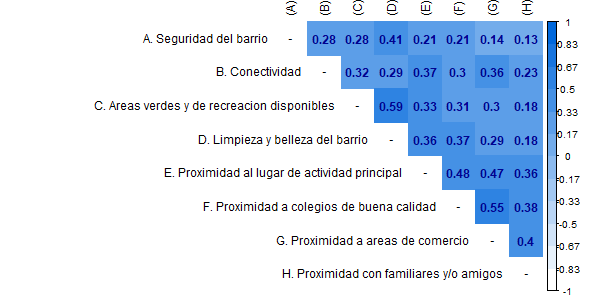
\includegraphics[width=1\linewidth,height=1\textheight]{output/graphs/satisfaccion-residencial_cor} 

}

\caption{Asociación indicadores satisfacción residencial.}\label{fig:unnamed-chunk-9}
\end{figure}

\hypertarget{capuxedtulo-ii}{%
\chapter{Capítulo II ---}\label{capuxedtulo-ii}}

\hypertarget{capuxedtulo-iii}{%
\chapter{Capítulo III ---}\label{capuxedtulo-iii}}

\hypertarget{bibliografuxeda}{%
\chapter*{Bibliografía}\label{bibliografuxeda}}
\addcontentsline{toc}{chapter}{Bibliografía}

\hypertarget{refs}{}
\leavevmode\hypertarget{ref-cepal_Cohesion_2021}{}%
CEPAL. (2021). \emph{Cohesión social y desarrollo social inclusivo en América Latina. Una propuesta normativa para una era de incertidumbres}.

\leavevmode\hypertarget{ref-coes_Radiografia_2019}{}%
COES. (2019). \emph{Radiografía del cambio social. Análisis de Resultados Longitudinales 2016-2018}.

\end{document}
